\documentclass[12pt, a4paper]{article}
\usepackage[margin=.8in]{geometry}
\usepackage{enumitem}
\usepackage{amssymb}
\usepackage{amsmath}
\usepackage{bm}
\usepackage{multicol}
\usepackage{graphicx}
\graphicspath{{./Figures/}}
\usepackage{color}
\usepackage{hyperref}
\hypersetup{
	colorlinks=true,
	linkcolor=blue,
	urlcolor=red,
}

\begin{document}
	\begin{titlepage}
		\begin{center} \Huge \textbf{Introduction to Statistics} \end{center}
		\tableofcontents
		\newpage
	\end{titlepage}

\begin{center} \section{Discrete Probability Distributions} \end{center}
	\subsection{Introduction}
	Informal Definition - A \textbf{random variable} is a quantitative variable whose value depends on chance in some way. \\~\\
	Suppose we about to toss a coin 3 times, let X represent the number of heads in 3 tosses. This means X is a random variable that will take on one of the values: 0,1,2,3 \\~\\
	\textbf{Discrete random variables} can take on a countable number of possible values (a finite of countably infinite number of possible values)\\~\\
	Examples of discrete random variables: \\
	i) The number of free throws an NBA player makes in his next 20 attempts.\\ \hspace*{5mm} Possible values: 0,1,...,20 \\
	ii) The number of rolls of a die needed to roll a 3 for the first time.\\ \hspace*{5mm} Possible values: 1,2,3,...\\
	iii) The profit on a \$1.50 bet on black in roulette. Possible values: -1.50,1.50 \\
	
	\noindent The \textbf{probability distribution} of a discrete random variable X is a listing of all possible values of X and their probabilities of occurring. \\
	
	\noindent ex: Approximately 60\% of full-term newborn babies develop jaundice. Suppose we sample 2 full-term newborn babies, and let X represent the number that develop jaundice. What is the probability distribution of X? \\
	Possible values of X: 0,1,2 and Possible outcomes: JJ, JN, NJ, NN. Respectively, the values of X are 2,1,1,0. So the probability of JJ = .6*.6, JN = NJ = .6*.4, NN = .4*.4
	\begin{minipage}[c]{7cm}
		$ p_X(x) =
		\begin{cases}
		.16   & \quad \text{if } x \text{ = 0}\\
		.48   & \quad \text{if } x \text{ = 1}\\
		.36   & \quad \text{if } x \text{ = 2}\\
		0	  & \quad {otherwise}
		\end{cases}$ \\~\\
	\end{minipage}
	\begin{minipage}[c]{7cm}
		Also can be written as a PMF: \\
		p(x) = $\binom{2}{x}0.6^x(1-0.6)^{2-x}$ for x = 0,1,2 \\
	\end{minipage}
	
	\noindent Notation: P(X = x) = p(x) which means the probability that the random variable (X) takes on a value of the random variable (x). \\~\\
	All discrete probability distributions must satisfy: \\
	1) 0 $\leq$ p(x) $\leq$ 1 for all x \\
	2) $\sum_{x}p(x)$ = 1 \\
	
	\subsection{Expected Value and Variance}
	The \textbf{expected value} \textit{(or expectation)} of a random variable si the theoretical mean of the random variable. We write this as \textbf{E[X] =} $\mathbf{\mu}$\\~\\
	To calculate the expected value of a discrete r.v. X: \\
	$\mathbf{E[X] = \sum_{x}x*p(x)}$ \newpage
	\noindent To calculate the expected value of a function g(X): \\
	$\mathbf{E[g(X)] = \sum_{x} g(x)*p(x)}$ \\~\\
	The \textbf{variance} of X can be thought of as the expectation of the squared distance of X from its mean. To calculate this we use: \\
	$\mathbf{\sigma^2 = E[(X - \mu)^2] = \sum_{x}(x-\mu)^2*p(x)}$ \\
	\hspace*{5.5mm}$\mathbf{= E[(X - \mu)^2] = E[X^2] - (E[X])^2 = E[X^2] - \mu^2}$ \\
	
	\noindent ex: Suppose you bought a novelty coin that has a probability of 0.6 of coming up H when flipped. Let X represent the number of H when the coin is tossed twice. \\~\\
	\begin{minipage}[c]{7cm}
		\begin{tabular}{ |c|c|c|c| } 
			\hline x & 0 & 1 & 2 \\ 
			\hline p(x) & 0.16 & 0.48 & 0.36 \\ 
			\hline
		\end{tabular}
	\end{minipage}
	\begin{minipage}[c]{7cm}
		What is E[X]? \\
		E[X] = $\sum x*p(x) \\ = 0*0.16 + 1*0.48 + 2*0.36$ = 1.2 \\
	\end{minipage}

	\noindent What is E[X$^2$]? \\
	= $\sum x^2*p(x) = 0^2*0.16 + 1^2*0.48 + 2^2*0.36$ = 1.92 \\~\\
	What is $\sigma^2$? \\
	$E[(X - \mu)^2] = \sum_{x}(x-\mu)^2*p(x) = (0-1.2)^2*0.16 + (1-1.2)^2*0.48 + (2-1.2)^2*0.36 = 0.48$ \\
	Or the easier way is using $E[X^2] - (E[X])^2$ = 1.92 - (1.2)$^2$ = 0.48 \\~\\
	
	\subsection{Bernoulli Distribution}
	ex: Toss a fair coin once, what is the distribution of the number of H? \\~\\
	Suppose we have: \\
	i) A single trial \\
	ii) The trial can result in one of two possible outcomes, labeled success and failure. \\
	iii) P(Success) = p, P(Failure) = (1 - p) \\~\\
	Let X = 1 if a success occurs, and X = 0 if a failure occurs. Then X has a Bernoulli distribution: \\
	$\mathbf{P(X=x) = p^x(1-p)^{1-x}}$ \textbf{for x = 0, 1} \\
	$\mathbf{\mu = E[X] = p}$ \\
	$\mathbf{\sigma^2 = p(1-p)}$ \\~\\
	ex: Approximately 1 in 200 American adults are lawyers. One American adult is randomly selected. What is the distribution of lawyers? \\
	We can see this is Bernoulli with p = $\frac{1}{200}$. so P(X=x) = $\frac{1}{200}^x(1-\frac{1}{200})^{1-x}$ \\
	P(X=1) = $\frac{1}{200}$ and P(X=0) = $\frac{199}{200}$ \\~\\
	NOTE: Some other common discrete probability distributions are built on the assumptions of independent Bernoulli trials: \\
	i) Binomial - Number of successes in n independent Bernoulli trials \\
	ii) Geometric - Number of trials to get first successes in independent Bernoulli trials \\
	iii) Negative Binomial -  Number of trials to get r$^{th}$ successes in independent Bernoulli trials \newpage
	
	\noindent \textbf{Deriving the Expectation:} \\
	E[X] = $\sum_x x*p(x) = 0*p^0(1-p)^{1-0} + 1*p^1(1-p)^{1-1} = 0(1-p) + 1*p = p$\\~\\
	\noindent \textbf{Deriving the Variance:} \\
	var(X) = $E[X^2] - (E[X])^2$ \\
	we find $E[X^2] = 0^2*p^0(1-p)^{1-0} + 1^2*p^1(1-p)^{1-1} = 0^2(1-p) + 1^2*p = p$ \\
	so $E[X^2] - (E[X])^2$ = p - p$^2$ = p(1-p) \\~\\
	
	\subsection{Binomial Distribution}
	We know the combinations formula (binomial coefficient): $\binom{n}{x} = \frac{n!}{x!(n-x)!}$ \\~\\
	Examples of problems that follow Binomial Distributions: \\
	i) Flip a coin 100 times, what is the probability H comes up at least 60 times? \\
	ii) You buy a certain type of lottery ticket once a week for 4 weeks, probability of winning a prize exactly twice? \\~\\
	The \textbf{binomial distribution} is the number of successes in n independent Bernoulli trials. \\~\\
	Conditions: \\
	i) There are n independent trials (tell us nothing above each other) \\
	ii) Each trial can result in one of two possible outcomes, labeled success and failure \\
	iii) P(Success) = p, and this stays constant from trial to trial. P(Failure) = 1-p \\
	iv) X represents the number of successes in n trials \\~\\
	Then X has a binomial distribution: \\
	$\mathbf{P(X=x) = \binom{n}{x}p^x(1-p)^{n-x}}$ \textbf{for x = 0,1,2,...,n} \\
	$\mathbf{\mu = E[X] = np}$ \\
	$\mathbf{\sigma^2 = np(1-p)}$ \\~\\
	ex: A balanced six-sided die is rolled 3 times, probability a 5 comes up exactly twice? \\
	Let X = the number of fives in 3 rolls, then X has a binomial distribution with n = 3 and p = $\frac{1}{6}$ so P(X=2) = $\binom{3}{2}(\frac{1}{6})^2(1-\frac{1}{6})^{3-2}$ = 0.0694 \\~\\	
	Why this formula: \\
	$p^x(1-p)^{n-x}$ is the probability of one specific ordering of successes and failures. There are $\binom{n}{x}$ possible orderings. \\~\\
	The \textbf{binomial random variable} cam be thought of as the sum of \textit{n} independent Bernoulli random variables, each with mean \textit{p} and variance \textit{p(1-p)}. \\~\\
	\noindent \textbf{Deriving the Expectation:} \\
	Let $U_1,...U_n$ be independent Bernoulli r.v. Then E[$U_i$] = p \\
	X = $U-1+...+U_n$ \\ E[X] = E[$U_1+...+U_n$] = E[X] = E[$U_1$] + ... + E[$U_n$] = p + ... + p \\
	As we see, we are summing p 'n' number of times, meaning that E[X] = np \newpage
	\noindent \textbf{Deriving the Variance:} \\
	Let $U_1,...U_n$ be independent Bernoulli r.v. Then var($U_i$) = p(1-p)
	X = $U-1+...+U_n$ \\ var(X) = var($U_1+...+U_n$) = var(X) = var($U_1$) + ... + var($U_n$) = p(1-p) + ... + p(1-p) \\
	As we see, we are summing p(1-p) 'n' number of times, meaning that var(X) = np(1-p) \\~\\	
	ex: According to Statistics Canada life tables, the probability a randomly selected 90 year-old Canadian male survives for at least another year is approx. 0.82. If twenty 90 year-old males are randomly selected. What is the probability exactly 18 survive for at least another year? \\
	We have n = 20 and p = 0.82, which can be written as X$\sim$B(20, 0.82) \\
	P(X=18) = $\binom{20}{18}0.82^{18}(1-0.82)^{20-18}$ = 0.173 \\~\\
	What is the probability that at least 18 survive? \\
	P(X $\geq$ 18) = P(X = 18) + P(X = 19) + P(X = 20) = $\binom{20}{18}0.82^{18}(1-0.82)^{20-18}$ + $\binom{20}{19}0.82^{19}(1-0.82)^{20-19}$ + $\binom{20}{20}0.82^{20}(1-0.82)^{20-20}$ = 0.173 + 0.083 + 0.019 = 0.275 \\~\\
	ex: The probability a randomly selected 40-year-old pregnant woman is carrying a fetus with down syndrome is approximately 0.01. Randomly select 25 40-year-old pregnant women, what is the probability exactly 2 are carrying a fetus with down syndrome?\\
	Let X = number of woman carrying babies with down syndrome, n = 25, p = 0.01 \\ P(X=2) = $\binom{25}{2}0.01^{2}(1-0.01)^{25-2} = 0.0238$ \\~\\
	ex: Suppose a six-sided die is rolled 16 times. What is the probability that on exactly 5 of the rolls, either a 3 or a 4 comes up? \\
	Redefine and let Success = 3 or 4, Failure = 1,2,5,6. n = 16, p = $\frac{2}{6}$ \\
	P(X=5) = $\binom{16}{5}(\frac{2}{6})^5(1-\frac{2}{6})^{16-5} = 0.2078$ \\~\\
	ex: A die is rolled until a 6 comes up 3 times. Let X represent the number of the trial on which the 3rd 6 appears. \\
	\textit{NOT} a binomial distribution, but rather the \textit{negative binomial distribution}. \\~\\
	ex: In a pool of 30 job applicants, 6 have a criminal record. You randomly select 8 from the 30 for an interview. What is the probability exactly 2 have a criminal record? \\
	\textit{NOT} a binomial distribution, knowing what happens in previous trials gives info about future trials (probability changes if first applicant select does have a criminal record). \\~\\
	ex: The number of putts a PGA tour player makes in his next 10 putts. \\
	\textit{NOT} a binomial distribution, not independent and the probability is always changing \\~\\
	ex: What is the probability there are exactly 8 lightning strikes in the first 5 minutes of the next thunderstorm? \\
	\textit{NOT} a binomial distribution, no fixed number of trials \newpage
	
	\subsection{Hypergeometric Distribution}
	ex: An urn contains 6 red balls and 14 yellow balls. 5 balls are randomly drawn without replacement, what is the probability exactly 4 red balls are drawn? \\
	Since they are drawn without replacement, they are not independent trials. So any sample of 5 balls is equally likely, so... P(Exactly 4 red balls) = $\frac{number\;of\;samples\;that\;result\;in\;4\;red\;and\;1\;yellow} {number\;of\;possible\;samples\;of\;size\;5}$ \\ = $\frac{\binom{6}{4}\binom{14}{1}}{\binom{20}{5}} = 0.01354$ \\~\\
	It is NOT appropriate to use the binomial distribution here because the sampling is done without replacement, therefore the trials are not independent. The probability is changing for each trial because if a red ball is drawn on the first try, the probability changes from $\frac{6}{20}$ to $\frac{5}{19}$ \\~\\
	Conditions: \\
	i) We are randomly sampling \textit{n} objects without replacement from a source that contains \\\hspace*{4mm} \textit{a} successes and \textit{N - a} failures. \\
	ii) X represents the number of successes in the sample. \\~\\
	Then X has the \textbf{hypergeometric distribution}: \\
	\textbf{$\mathbf{P(X=x) = \frac{\binom{a}{x}\binom{N-a}{n-x}}{\binom{N}{n}}}$} for x = Max(0, n-(N-a)),..., Min(a,n) \\
	NOTE: n-(N-a) is the number of samples (n) - the number of failures in the pop (N-a) \\
	$\mathbf{\mu = n \frac{a}{N}}$ \\~\\
	ex: Suppose a large high school has 1100 female students and 900 males students. A random sample of 10 students is drawn, what is the probability exactly 7 of the students are female? (Sampling is done without replacement) \\
	Let X = number of female students selected, n = 10, a = 1100, N = 2000, x = 7, \\
	so P(X=7) = $\frac{\binom{1100}{7}\binom{900}{3}}{\binom{2000}{10}}$ = 0.16649 \\~\\
	
	\noindent The binomial distribution can sometimes provide a reasonable approximation to the hypergeometric distribution (if we are not sampling a large proportion of the population). Rough Guideline: if we are not sampling more than 5\% of the population, the binomial provides a reasonable approximation. \\~\\	
	\noindent ex: Suppose a business employs 12 Democrats, 24 Republicans, and 8 independents. IF a random sample of 6 employees is drawn, what is the probability there are 3 Democrats, 2 Republicans, and 1 independent in the sample? \\
	We can extend this formula, so that $\frac{\binom{12}{3}\binom{24}{2}\binom{8}{1}}{\binom{44}{6}} = 0.0688$ \\~\\
	
	\subsection{Poisson Distribution}
	Suppose we are counting the number of occurrences of an event in a given unit of time, distance, area, or volume. For example, the number of car accidents in a day or the number of dandelions in a square meter plot of land. \newpage
	\noindent Conditions: \\
	i) Events are occurring independently. \\
	ii) Probability that an event occurs in a given length of time does not change though time. \\~\\
	Then X, the number of events in a fixed unit of time, has the \textbf{Poisson Distribution}: \\
	$\mathbf{P(X = x) = \frac{\lambda^xe^{-\lambda}}{x!}}$ for x = 0,1,2,.. (with $\lambda$ = np)\\
	$\mathbf{\mu = \lambda}$ \\
	$\mathbf{\sigma^2 = \lambda}$ \\~\\
	ex: One nanogram of Plutonium-239 will have an average 2.3 radioactive decays per second, and the number of decays will follow a Poisson distribution. What is the probability that in a 2 second period there are exactly 3 radioactive decays? \\
	Let X = the number of decays in a 2 second period, $\lambda$ = 2.3*2 = 4.6 \\
	so P(X=3) = $\frac{4.6^3e^{-4.6}}{3!} = 0.163$ \\~\\
	What is the probability there are no more than 3 radioactive decays? \\
	P(X $\leq$ 3) = P(X=0) + P(X=1) + P(X=2) + P(X=3) \\\
	= $\frac{4.6^0e^{-4.6}}{0!} + \frac{4.6^1e^{-4.6}}{1!} + \frac{4.6^2e^{-4.6}}{2!} + \frac{4.6^3e^{-4.6}}{3!}$ = 0.01 + 0.046 + 0.106 + 0.163 = 0.326 \\~\\
	
	\subsection{Relationship between Binomial and Poisson Distributions}
	- The binomial distribution tends toward the Poisson distribution as \textit{n} $\rightarrow$ $\infty$, \textit{p} $\rightarrow$ 0, and \textit{np} stays constant. \\
	- The Poisson distribution with $\lambda$ = \textit{np} closely approximates the binomial distribution if \textit{n} if large and \textit{p} is small \\~\\
	The Poisson distribution is typically used as an approximation to the true underlying reality. It can be difficult to determine whether a r.v. has a Poisson distribution. \\~\\	
	ex: Albinism is a rare genetic disorder that affects one in 20,000 Europeans. People with albinism produce little or none of the pigment melanin. In a random sample of 1000 Europeans, what is the probability exactly 2 have albinism? \\~\\
	This is a binomial distribution with n = 1000, p = $\frac{1}{20000}$ so we get ...\\
	P(X=2) = $\binom{1000}{2} \frac{1}{20000}^2(1-\frac{1}{20000})^{1000-2}  = 0.001187965$ \\
	Now let this follow a Poisson distribution with $\lambda$ = np = 1000*$\frac{1}{20000}$ = 0.05 \\
	P(X=2) = $\frac{0.05^2e^{-0.05}}{2!} = 0.001189037$\\~\\
	Rough Guideline: \\
	The Poisson approximation is a \textit{reasonable} if n $>$ 50 and np $<$ 5 \\~\\
	Why use this approximation:\\
	i) The factorials and exponential in the binomial formula can become problematic to calculate. \\
	ii) A problem may be binomial conceptually, but \textit{n} and \textit{p} may be unknown (we may only know the mean). \\~\\
	
	\subsection{Geometric Distribution}
	The \textbf{geometric distribution} is the distribution of the number of trials needed to get the first success in repeated Bernoulli trials. \\~\\
	Conditions: \\
	i) There are independent trials \\
	ii) Each trial results in one of two possible outcomes, labeled success and failure. \\
	iii) P(Success) = p, and stays constant from trial to trial. P(Failure) = 1-p \\
	iv) X represents the number of trials need to get the first success \\~\\
	For the first success to occur on the xth trial: \\
	1) The first x-1 trials must be failures. (1-p)$^{x-1}$\\
	2) The xth trial must be a success (p) \\~\\
	$\mathbf{P(X=x) = (1-p)^{x-1}p}$ for x = 1,2,3,.. \\
	$\mathbf{\mu = \frac{1}{p}}$ \\
	$\mathbf{\sigma^2 = \frac{1-p}{p^2}}$ \\~\\
	NOTE: Geometric distribution always shows right skewness when graphed (left-side heavy)\\~\\
	ex: In a large population of adults, 30\% have received CPR training. IF adults from the pop are randomly selected, what is the probability that the 6th person sampled is the first that has received CPR training? \\
	p = 0.3, X = 6th person sampled has had training, so... \\
	P(X=6) = $(1-.03)^{6-1}0.3 = 0.0504$ \\
	
	\noindent What is the probability that the first person trained in CPR occurs on or before the third person sampled? \\
	P(X$\leq$3) = P(X=1) + P(X=2) + P(X=3) = $0.7^0*0.3 + 0.7^1*0.3 + 0.7^2*0.3 = 0.657$ \\~\\
	Cumulative Distribution Function: \\
	$\mathbf{F(x) = P(X \leq x) = 1 - (1-p)^x}$ for x = 1,2,3,... \\~\\
	so for the above example, P(X$\leq$3) = 1 - (.7)$^3$ = 0.657 \\~\\
	
	\subsection{Negative Binomial Distribution}
	The \textbf{negative binomial distribution} is the distribution of the number of trials to get the rth success in repeated Bernoulli trials. It is the number of trials needed to get a fixed number of successes \\~\\
	Conditions: \\
	i) We have independent trials \\
	ii) Each trial results in one of two possible outcomes, labeled success and failure. \\
	iii) P(Success) = p, and stays constant from trial to trial. P(Failure) = 1-p \\
	iv) X represents the trial number of the rth success \\~\\
	For the rth success to occur on the xth trial: \\
	1) The first x-1 trials must result in r-1 successes. $\binom{x-1}{r-1}p^{r-1}(1-p)^{(x-1)-(r-1)}$ \\
	2) The xth trial must be a success, which has a probability of p \\~\\
	Then the probability the rth success occurs on the xth trial is: \\
	From above we know $p*\binom{x-1}{r-1}p^{r-1}(1-p)^{(x-1)-(r-1)}$ so... \\
	$\mathbf{P(X=x) = \binom{x-1}{r-1}p^{r}(1-p)^{(x-r)}}$ for x = r,r+1,... \\
	$\mathbf{\mu = \frac{r}{p}}$ \\
	$\mathbf{sigma^2 = \frac{r(1-p)}{p^2}}$ \\~\\
	ex: A person conducting telephone surveys must get 3 more completed surveys before their job is finished. One each randomly dialed number, there is a 9\% chance of reaching an adult who will completed the survey. What is the probability that the 3rd completed survey occurs on the 10th call? \\
	p = 0.09, r = 3, x = 10, so... P(X=10) = $\binom{10-1}{3-1}0.09^3(1-0.09)^{10-3} = 0.01356$ \\
	$\mu = \frac{3}{0.09} = 33.333$ \\~\\
	
	\subsection{Multinomial Distribution}
	The \textbf{multinomial distribution} is a generalization of the binomial distribution. The number of outcomes can be greater than 2. \\~\\
	Conditions: \\
	i) We have independent trials \\
	ii) Each trial results in one of \textit{k} mutually exclusive outcomes. \\
	iii) On any single trial, these \textit{k} outcomes occur with probabilities $p_1,...,p_k$ ($\sum_{i=1}^{k}p_i = 1$) \\~\\
	Let the random variable $X_i$ represent the number of occurrences of outcome \textit{i} (where i = 1,...,k). Then... \\
	$\mathbf{P(X_1 = x_1,...,X_k = x_k) = \frac{n!}{x_1!...x_k!}p_1^{x_1}...p_k^{x_k}}$ for $x_i = 0,1,...,n$ (where $\sum_{i=1}^{k}x_i = n$)\\
	$\mathbf{E[X_i] = np_i}$ \\
	$\mathbf{var(X_i) = np_i(1-p_i)}$\\~\\
	ex: In a random sample of 10 Americans, waht is the probability 6 have blood type O, 2 have A, 1 has B, and 1 has AB? \\~\\
	\begin{minipage}[c]{7cm}
		\begin{tabular}{ |c|c|c|c|c| } 
			\hline Type & O & A & B & AB \\ 
			\hline Prob & 0.44 & 0.42 & 0.10 & 0.04 \\ 
			\hline
		\end{tabular}
	\end{minipage}
	\begin{minipage}[c]{7cm}
		P($X_1 = 6, X_2 = 2, X_3 = 1, X_4 = 1$) \\
		= $\frac{10!}{6!2!1!1!}0.44^6\,0.42^2\,0.10^1\,0.04^1 =0.0129$
	\end{minipage} \\~\\
	
	\noindent ex: An urn contains 8 red balls, 3 yellow balls, 9 white balls. 6 balls are randomly chosen \textit{with replacement}. What is the probability 2 are red, 1 is yellow, and 3 are white? \\
	P($X_1 = 2, X_2 = 1, X_3 = 3$) = $\frac{6!}{2!1!3!}(\frac{8}{20})^2(\frac{3}{20})^1(\frac{9}{20})^3 = 0.13122$ \\~\\
	If the sampling above was done WITHOUT replacement, it would not have satisfied the multinomial distribution (different probabilities for each draw) and we would use the multivariate hypergeometric distribution. (example below)\\
	
	\noindent ex: An urn contains 8 red balls, 3 yellow balls, 9 white balls. 6 balls are randomly chosen \textit{without replacement}. What is the probability 2 are red, 1 is yellow, and 3 are white?
	P($X_1 = 2, X_2 = 1, X_3 = 3$) = $\frac{\binom{8}{2}\binom{3}{1}\binom{9}{3}}{\binom{20}{6}} = 0.18204 $ \\~\\
	
	\subsection{Overview and Examples}
	\textbf{Bernoulli}: \\
	The distribution of a number of successes on a single Bernoulli trial (p,1-p). \\~\\
	\textbf{Binomial}: \\
	The distribution of the number of successes in \textit{n} independent Bernoulli trials (p,1-p). \\
	The number of trials is fixed, and the number of successes is a random variable. \\~\\
	\textbf{Geometric}: \\
	The number of trials needed to get the first success in a sequence of independent Bernoulli trials. \\~\\
	\textbf{Negative Binomial}: \\
	The distribution of the number of trials needed to get a certain number of successes in a sequence of independent Bernoulli trials. \\
	The number of successes is fixed, and the number of trials is a random variable. \\~\\
	\textbf{Hypergeometric}: \\
	The distribution of the number of successes when we are drawing without replacement (thus not independent trials) from a source with a certain amount of successes and a certain amount of failures. \\
	NOTE: The binomial distribution can approximate the hypergeometric if we are only sampling a small fraction of the population \\~\\
	\textbf{Poisson}: \\
	The distribution of the number of events in a given time, length, area, or volume if those events are occurring randomly and independently. \\
	
	\noindent \textbf{All Distributions Examples}: \\
	ex: For a military mission, engineers are creating an expensive system that relies on an important component. This component is very delicate and fragile has a probability of failure of 0.32. They install 6 of these components in parallel, in such a way that they work independently. If any one of these components works, the system works. What is the probability that exactly 1 of these components works? \\
	Let X = number of working components, p = 0.68, 1-p = 0.32, n = 6 \\
	P(X=1) = $\binom{6}{1}.68^1(.32)^5 = 0.0137$ \\~\\
	Part 2, what is the probability that at least 1 of the 6 components work? \\
	P(X$\geq$1) = 1 - P(X=0) = 1 - $\binom{6}{0}.68^0(.32)^6$ = 1 - 0.00107 = 0.99893 \newpage
	\noindent ex: A certain union chapter has 32 male and 26 female members. An important committee of 7 people needs to be struck, the president says they will randomly select 7 of the members. What is the probability there are exactly 6 women on the committee? \\
	Let X = number of women chosen for the committee, we see the sampling is done without replacement. 
	So it follows the hypergeometric distribution, P(X=6) = $\frac{\binom{26}{6}\binom{32}{1}}{\binom{58}{7}} = 0.0245$ \\~\\
	Part 2, what is the probability the committee contains at least 6 women? \\
	P(X$\geq$6) = P(X=6) + P(X=7) = $\frac{\binom{26}{6}\binom{32}{1}}{\binom{58}{7}} + \frac{\binom{26}{7}\binom{32}{10}}{\binom{58}{7}} = 0.0267$ \\~\\
	ex: Suppose a beverage manufacturer puts tiny gold flakes into a beverage container, at an average rate of 800 flakes per one liter container. A one liter container is randomly selected, shaken, and a 10 ml sample is drawn. What is the probability it contains exactly 2 flakes of gold? \\
	Let X = the number of gold flakes in the 10 ml sample, since its volume we have Poisson \\
	$\lambda = \frac{10}{1000}*800 = 8$, meaning we have P(X=2) = $\frac{8^2e^{-8}}{2!} = 0.0107$ \\~\\	
	\noindent A European roulette wheel has 18 red slots, 18 black lots, 1 green slot. It is reasonable to assume that the ball is equally likely to land in any of the 37 slots, what is the probability that the first time the ball lands in a red slot occurs on the 5th spin? \\
	Let X = the number of spins need to get first red \\ we can see it will be geometric with p = $\frac{18}{37}$ so,
	P(X=5) = (1-$\frac{18}{37})^4\frac{18}{37}$ = 0.0338 \\~\\
	Part 2, what is the probability the first time the ball lands in a red slots occurs at some point after the 6th spin? \\
	P(X$>$6) = P(X=7) + P(X=8) + ... = 1 - P(X$\leq$6). To solve this, we see that the first 6 spins are not red, so the first red must happen after the 6th spin. \\ P(X$>$) = (1 - $\frac{18}{37})^6 = 0.0183$ \\~\\
	ex: Tom is part of a production process that makes an expensive piece of equipment. If tom makes a mistake, the equipment is destroyed at a high cost to the manufacturer. He has probability of 0.001 of destroying an individual piece of equipment, but if he destroys one piece he gets rattled and is more likely to destroy other pieces. What is the probability that Tom destroys exactly 3 of the next 20 items he works on? \\
	NOT ANSWERABLE WITH THE GIVEN INFORMATION \newpage
	


\begin{center} \section{Continuous Probability Distributions} \end{center}
	\subsection{Introduction}
	\textbf{Continuous random variables} can take on an infinite number of possible values, corresponding to every value in an interval. We cannot model continuous random variables with the same methods we used for discrete random variables.\\~\\
	\textbf{Probability Density Function (PDF)} is the model used for a continuous random variable with curve f(x). \\~\\
	NOTE: For continuous random variables, areas are simply the area under the curve. \\~\\
	We know that P(a$<$X$<$b) is the area under the portion of the curve (a,b), but \\ P(X=a) = 0 since the area of any single point is equal to 0. \\~\\
	For any continuous probability distribution: \\
	i) f(x) $\geq$ 0 for all x \\
	ii) The are under the entire curve is equal to one. \\~\\
	There are a number of common continuous probability distributions that come up frequently in theory and practice such as \textit{normal, uniform, and exponential} \\~\\
	Probabilities and percentiles are found by integrating the probability density function (deriving the mean and variance also requires integration). \\~\\
	
	\subsection{Finding Probabilities and Percentiles}
	Properties of a legitimate PDF: \\
	1) It can never take on negative values \\
	2) The area under the curve must equal one, such that $\mathbf{\int_{-\infty}^{\infty} f(x)dx = 1}$ \\~\\
	To find the median: $\mathbf{\int_{-\infty}^{m}f(x)\;dx = \frac{1}{2}}$ \\~\\
	To find the Cumulative Distribution Function (CDF): F(x) = P(X$\leq$x) = $\mathbf{\int_{-\infty}^{x}f(t)\;dt}$ \\~\\
	ex: Suppose for a random variable X: f(x) = cx$^3$ for 2 $\leq$x$\leq$4 and 0 otherwise. What value of \textit{c} makes this a legitimate probability distribution? \\
	$1= \int_{2}^{4} cx^3\; dx = \frac{cx^4}{4} \bigr|_2^4 = c(\frac{4^4}{4}-\frac{2^4}{4}) = 60c$ which means c = $\frac{1}{60}$ \\~\\
	What is P(X$>$3) for f(x) = $\frac{1}{60}x^3$ for 2 $\leq$x$\leq$4? \\
	$1 = \int_{3}^{4}\frac{1}{60}x^3\; dx = \frac{1}{60}\frac{x^4}{4} \bigr|_3^4 = \frac{1}{60}(\frac{4^4}{4}-\frac{3^4}{4}) = \frac{175}{240} = 0.729$ \\~\\
	What is the median of f(x) = $\frac{1}{60}x^3$ for 2 $\leq$x$\leq$4? \\
	$\frac{1}{2} = \int_{2}^{m}\frac{1}{60}x^3\; dx = \frac{1}{60}\frac{x^4}{4} \bigr|_2^m = \frac{1}{60}(\frac{m^4}{4}-\frac{2^4}{4}) = \frac{m^4 - 2^4}{240}$ so $\frac{m^4 - 2^4}{240} = \frac{1}{2}$ which means m$^4$ = 136 so m $\approx$ 3.415 \newpage
	
	\noindent What is the CDF of f(x) = $\frac{1}{60}x^3$ for 2 $\leq$x$\leq$4? \\
	$\int_2^x \frac{1}{60}t^3\;dt = \frac{1}{60}\frac{t^4}{4}\bigr|_2^x = \frac{1}{60}(\frac{x^4}{4}-\frac{2^4}{4})$ so our F(x) is... \\
	$ F(x) =
		\begin{cases}
		0   & \quad \text{if } x<2\\
		\frac{x^4 - 2^4}{240}   & \quad \text{2$\leq$x$\leq$4}\\
		1	& \quad \text{if } x>4
		\end{cases}$ \\~\\
		
	\noindent What is P(X$\leq$2.7)? \\
	We know using out F(x) found above we can plug 2.7 in, so $\frac{2.7^2-2^4}{240} = 0.155$ \\~\\
	
	\subsection{Mean and Variance of Continuous R.V.}
	To find the mean: \textbf{E[X] = $\mu = \mathbf{\int_{-\infty}^{\infty}xf(x)\;dx}$} \\~\\
	To find the variance: \textbf{var(X) = $\mathbf{\sigma^2 = E[(X-\mu)^2] = \int_{-\infty}^{\infty}(x-\mu)^2f(x)\;dx}$} \\
	\hspace*{64mm} = \textbf{E[X$^2$] - (E[X])$^2$ = $\mathbf{\int_{-\infty}^{\infty}x^2f(x)\;dx}$ - (E[X])$^2$} \\~\\
	ex: What is the E[X] of f(x) = $\frac{1}{60}x^3$ for 2 $\leq$x$\leq$4? \\
	$\int_{2}^{4}x*\frac{1}{60}x^3 = \frac{1}{60}*\frac{x^5}{5}\bigr|_2^4 = \frac{1}{60}(\frac{4^5}{5}-\frac{2^5}{5}) = \frac{992}{300} \approx 3.3$ \\~\\
	ex: What is the var(X) of f(x) = $\frac{1}{60}x^3$ for 2 $\leq$x$\leq$4? \\
	E[X$^2$] = $\int_{2}^{4}x^2*\frac{1}{60}x^3 = \frac{1}{60}*\frac{x^6}{6}\bigr|_2^4 = \frac{1}{60}(\frac{4^6}{6}-\frac{2^6}{6}) = \frac{4032}{360} = \frac{56}{5}$ \\ so E[X$^2$] - (E[X])$^2$ = $\frac{56}{5} - \frac{248}{75}^2 = \frac{1496}{5625} \approx 0.266$ \\~\\
	
	\subsection{Continuous Uniform Distribution}
	For the uniform distribution, f(x) is constant over the possible values of x. \\~\\
	The PDF of the uniform distribution: \\
	$ \mathbf{f(x) =
	\begin{cases}
	\frac{1}{d-c}   & \quad \textbf{for c$\leq$x$\leq$d}\\
	0	& \quad \textbf{elsewhere }
	\end{cases}}$ \\~\\
	The mean of the uniform distribution: \textbf{E[X]} = $\mathbf{\mu = \frac{c+d}{2}}$ (same for median) \\~\\
	The variance of the uniform distribution: \textbf{var(X)} $\mathbf{= \frac{1}{12}(d-c)^2}$ \\~\\
	For the uniform distribution, areas under the curve are simply rectangles (but still continuous) and can be found by taking the area of the rectangle rather than integration. \\~\\
	ex: Part 1, suppose X is a random variable that has a uniform distribution with \\ c = 200 and d = 250. What is f(x)? \\
	f(x) = $\frac{1}{250-200} = \frac{1}{50}$ for 200 $\leq$ x $\leq$ 250, and 0 otherwise \newpage
	
	\noindent Part 2, what is P(X$>$ 230)? \\
	= (250-230)*$\frac{1}{50} = 0.4$ \\~\\
	Part 3, what is the 20th percentile of this distribution? \\
	We need to find the value of the variable for which the area to the left is 0.2 (call it 'a'). \\
	= (a-200)*$\frac{1}{50}$ which must equal .2 so, a-200 = 10, then a = 210 \\~\\
	
	\subsection{Normal (Gaussian) Distribution}
	The probability density function (PDF) is: \\
	$\mathbf{f(x) = \frac{1}{\sqrt{2\pi}\sigma}e^{-\frac{1}{2\sigma^2}(x-\mu)^2}}$ where $-\infty < x,\mu < \infty$ and $\sigma >$0 \\~\\
	The distribution will be symmetric about $\mu$, since it will always be the center, and is also the median. \\~\\
	We also know that $\approx$ 68\% of the area lies within $\pm\sigma$ of $\mu$, $\approx$ 98\% of the area lies within $2\pm\sigma$ of $\mu$, and $\approx$ 99.7\% of the area lies within $3\pm\sigma$ of $\mu$. \\~\\
	We can see (graphing) that when the standard deviation becomes larger, there is more area in the tails and a lower peak on the graph. \\~\\
	Notation: \\
	If X is a random variable that has a normal distribution with mean $\mu$ and variance $\sigma^2$, we write this as:
	$\mathbf{X\sim N(\mu,\sigma^2)}$ \\~\\
	The standard normal distribution is a normal distribution with mean 0 and variance 1, written Z$\sim$N(0,1) \\~\\
	Finding probabilities and percentiles requires integrating the PDF (we can use a standard normal table to find these values). \\~\\
	
	\subsection{Standardizing Normally Distributed R.V.}
	The standard normal distribution is a normal distribution with $\mu$ = 0 and $\sigma$ = 1 \\~\\
	Suppose X is a normally distributed random variable with mean $\mu$ and standard deviation $\sigma$, then X $\sim(\mu,\sigma^2)$. Then to transform this distribution: \\ Z = $\frac{X-\mu}{\sigma}$ such that Z $\sim$ N(0,1) \\~\\
	ex: Suppose the height of adult American females is approx. normally distributed with a mean of 162.2 cm and a standard deviation of 6.8 cm. What is the probability a randomly selected adult American female is taller that 170.5 cm? \\
	Then let P(X$>$170.5) = P($\frac{X-\mu}{\sigma}>\frac{170.5-\mu}{\sigma}$) = P(Z $>\frac{170.5-162.2}{6.8}$) = P(Z$>$1.22) = 0.111 (by using a standard normal table) \newpage
	
	\noindent What is the probability a randomly selected adult American female has a height between 150.5 and 170.5 cm? \\
	P(150.5$<$X$<$170.5) = P($\frac{150.5-\mu}{sigma}<\frac{X-\mu}{\sigma}<\frac{170.5-\mu}{\sigma}$) = P($\frac{150.5-162.2}{6.8}<Z<\frac{170.5-162.2}{6.8}$) \\ = P(-1.72$<$Z$<$1.22) = 0.846 \\~\\
	What is the 10th percentile of the height of adult females? \\
	From a standard normal table, we see the 10th percentile of a standard normal curve is -1.28. Since Z = $\frac{x-\mu}{\sigma}$ so X = $\mu + \sigma Z$ which means X = 162.2 + 6.8(-1.28) = 153.5 \\~\\
	
	\subsection{Normal Approximation to the Binomial Distribution}
	The continuous normal distribution can sometimes be used to approximate the discrete binomial distribution. \\~\\
	We would want to do this because the normal approximation is often used in statistical inference. \\~\\
	The binomial distribution is perfectly symmetric if p = 0.5, and has some skewness when p $\neq$ 0.5. So, the normal approximation works best when p us close to 0.5, and when \textit{n} is large. \\~\\
	Rough Guideline: \\
	The normal approximation is reasonable is both np $\geq$ 10 and n(1-p) $\geq$ 10. \\~\\
	For a binomial random variable X: \\
	$\mu$ = np, $\sigma^2$ = np(1-p) \\~\\
	ex: Let X be a binomial random variable with n = 75 and p = 0.6. What is $\mu$, $\sigma^2$, and P(X$\geq$52)? \\
	$\mu$ = np = 75*0.6 = 45, $\sigma^2$ = np(1-p) = 76*0.6(1-0.6) = 18, then $\sigma$ = $\sqrt{18}$ \\ P(X$\geq$52) = P(Z$\geq\frac{52-45}{\sqrt{18}}$) = P(Z $\geq$ 1.645) = 0.0495. However, if we use the binomial distribution to find the answer we get exactly 0.0611 (we can improve our estimate) \\~\\
	We can improve the approximation with a \textbf{continuity correction} (move from discrete to continuous distribution) \\~\\
	ex: What is P(X$\geq$52), P(X$>$52), P(X $\leq$ 52), and P(X$<$52)? \\
	P(X$\geq$52) = P(Z$\geq \frac{51.5-45}{\sqrt{18}}$) = P(Z$\geq$1.532) = 0.0628 \\
	P(X$>$52) = P(Z $>\frac{52.5-45}{\sqrt{18}}$) = P(Z$>1.768$) = 0.0385 \\
	P(X $\leq$ 52) = P(Z $\leq\frac{52.5-45}{\sqrt{18}}$) = P(Z $\leq$1.768) = 0.9615 \\
	P(X$<$52) = P(Z $\leq\frac{51.5-45}{\sqrt{18}}$) = P(Z$<$1.532) = 0.9372 \\~\\
	The results of the continuity correction are: \\
	For P(X $\geq$52): No CC = 0.0495, CC = 0.0628, Exact = 0.0611 \\
	For P(X $>$ 52): No CC = 0.0485, CC = 0.0385, Exact = 0.0367 \newpage
	
	\subsection{Introduction to Chi-Square Distribution}
	The $\chi^2$ distribution is a continuous probability distribution that is widely used in statistical inference. \\~\\
	The $\chi^2$ distribution is related to the standard normal distribution: \\
	- If a random variable Z has the standard normal distribution then $Z^2$ has the $\chi^2$ distribution with one degree of freedom. \\~\\
	If $Z_1, Z_2, ..., Z_k$ are independent standard normal random variables, then \\
	$Z_1^2 + Z_2^2 + ...+ Z_k^2$ has a $\chi^2$ distribution with \textit{k} degrees of freedom \\~\\
	The PDF of the $\chi^2$ distribution with \textit{k} degrees of freedom: \\
	\large $\mathbf{f(x) = \frac{x^{k/2-1}e^{-x/2}}{2^{k/2}\Gamma(k/2)}}$ \normalsize for x $\geq$ 0 \\
	$\mathbf{\mu = k}$ \\
	$\mathbf{\sigma^2 = 2k}$ \\~\\
	As degrees of freedom increases, the graph moves from being skewed left towards the center since $\mu$ = k, it will be highest at this value since \textit{k} is the degrees of freedom. \\~\\
	Areas and percentiles for $\chi^2$ distribution are found by software or a $\chi^2$ table \\~\\
	
	\subsection{Introduction to Student t Distribution}
	The t distribution is an important continuous probability distribution that is widely used in statistical inference and is strongly related to the standard normal distribution. \\~\\
	Conditions: \\
	i) Z has the standard normal distribution \\
	ii) U has the $\chi^2$ distribution with $\nu$ degrees of freedom \\
	iii) Z and U are independent \\~\\
	Then we get \large \textbf{T = } $\mathbf{\frac{Z}{\sqrt{\frac{U}{\nu}}}}$ \normalsize that has $\nu$ degrees of freedom \\~\\
	If we are drawing \textit{n} independent observations from a normally distributed population with mean $\mu$ and variance $\sigma^2$, then: \\
	\Large $\mathbf{\frac{\bar{X} - \mu}{S/\sqrt{n}}}$ \normalsize with n-1 degrees of freedom \\
	where $\bar{X}$ is the sample mean of n observations \\
	S is the sample standard deviation of n observations \\~\\
	The t distribution often arises in statistical inference on means, when we are sampling from a normally distributed population. \newpage
	
	\noindent The PDF of the t distribution with $\nu$ degrees of freedom: \\
	\Large $\mathbf{f(t) = \frac{\Gamma(\frac{\nu+1}{2})}{\sqrt{\nu\pi}\Gamma(\frac{\nu}{2})}(1+\frac{t^2}{\nu})^{-\frac{\nu+1}{2}}}$ \normalsize for $-\infty < t < \infty$ \\
	- $\Gamma$ is the gamma function \\
	- $\nu >$ 0 \\
	- The median = 0 \\
	- $\mu = $ 0 for $\nu >$ 1, otherwise $\mu$ is undefined \\
	- $\sigma^2$ = $\frac{\nu}{\nu-2}$ for $\nu >$ 2 \\~\\
	As the degrees of freedom increase, the t distribution tends towards the standard normal distribution. This is because the median is 0 and $\mu$ is 0. The t distribution with 20 degrees of freedom is very similar to the standard normal distribution, but does have slightly more area in the tails. \\~\\
	Areas and percentiles for the t distribution are found by software or a t table \\~\\ 
	
	\subsection{Introduction to the F Distribution}
	The F distribution is related to the $\chi^2$ distribution \\~\\
	Conditions: \\
	i) $U_1$ has a $\chi^2$ distribution with $\nu_1$ degrees of freedom. \\
	ii) $U_2$ has a $\chi^2$ distribution with $\nu_n$ degrees of freedom. \\~\\
	This means \large \textbf{F = } $\mathbf{\frac{U_1/ \nu_1}{U_2/ \nu_2}}$ \normalsize with $\nu_1, \nu_2$ degrees of freedom \\~\\
	Implication: \\
	The F distribution often arises when we are working with ratios of variance. \\~\\
	$\mathbf{\mu = \frac{\nu_2}{\nu_2 - 2}}$ for $\nu_2 >$ 2 \\
	If degrees of freedom for $\nu_1$ and $\nu_2$ are equal, then median is 1. \\~\\
	Areas and percentiles for the F distribution are found by software or a F table \newpage
	

\begin{center} \section{Using Tables to Find Areas and Percentiles} \end{center}
	\subsection{Area/Percentiles (Tables for area left of z)}
	\begin{minipage}[c]{8.5cm}
		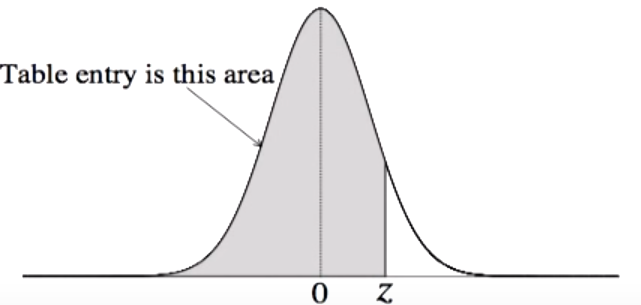
\includegraphics[scale=.45]{leftz} \\
	\end{minipage}
	\begin{minipage}[c]{6cm}
		NOTE: This is for tables that give area to the left of z \\~\\
	\end{minipage} \\~\\
	NOTE: For continuous random variable, P(Z$<$z) and P(Z$\leq$z) are the same since \\ P(Z=z) = 0 for any single point since probabilities is equal to area. \\~\\
	ex: Suppose Z is a r.v. with a standard normal distribution. What is P(Z$<$1.43)? \\
	Using a table we see it = 0.9236 \\~\\
	ex: Suppose Z is a r.v. with a standard normal distribution. What is P(Z$>$1.43)? \\
	From above problem we got P(Z$<$1.43) = 0.9236, so just do 1-0.9236 = 0.0764 \\~\\
	ex: What is P(-1.28$\leq$Z$\leq$0.72)? \\
	We will do P(Z$\leq$0.72) - P(Z$\leq$-1.28) = 0.7642 - 0.1003 = 0.6639 \\~\\
	We get the formula: \\
	$\mathbf{P(z_1\leq Z \leq z_2) = P(Z\leq z_2) - P(Z\leq z_1)}$ \\~\\
	ex: Suppose Z is a random variable with a standard normal distribution. What is the value $z_0$ such that P(Z$<z_0$) = 0.6331? \\ Looking at a table (in the area section) we see that this value = 0.34. \\~\\
	ex: What is the value $z_0$ such that P(Z$>z_0$) = 0.9838? \\
	Since our table gives us the area to the left, we do 1-0.9838 = 0.0162. From here, look at the table to find P(Z$<$0.0162) = -2.14. So we see $z_0$ = -2.14 \\~\\
	ex: What is the value $z_0$ such that P($-z_0 < Z < z_0$) = 0.95? \\
	We know the area between the two points is 0.95, so the area of both tails is 0.05. Knowing it is evenly distributed, we can see that each tail has an area of $\frac{0.05}{2}$ = 0.025. From this, we see that the area to the left of $z_0$ is 0.975 and the area to the left of -$z_0$ is 0.025. Looking at the table, we can see the z value that gives us an area = 0.975 is 1.96. So our $z_0$ value = 1.96. \\~\\
	ex: What is the 60th percentile of the standard normal distribution? \\
	This means what z value gives us area = 0.6 to the left. Looking at a table, the closest value in the table is 0.25. So our 60th percentile is $\approx$ 0.25 \newpage
	
	\subsection{Area/Percentiles (Tables for area between 0 and z)}
	\begin{minipage}[c]{8.5cm}
		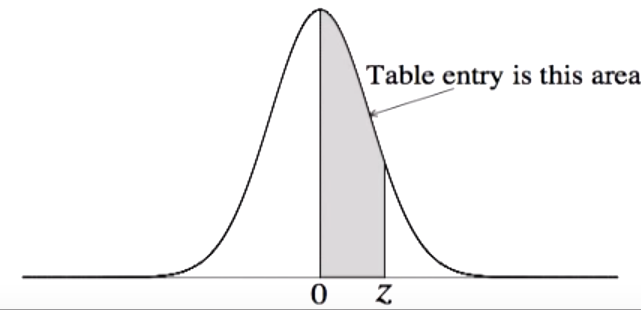
\includegraphics[scale=.45]{betwn} \\
	\end{minipage}
	\begin{minipage}[c]{6cm}
		NOTE: This is for tables that give area between 0 and z \\~\\
	\end{minipage} \\~\\
	ex: Suppose Z is a r.v. with a standard normal distribution. What is P($0<Z<1.43$)? \\
	Looking at a table, we can see the value we get is = 0.4236 \\~\\
	ex: What is P(Z$>$1.43)? \\
	Since our probabilities are split evenly, we know that 0.5 of the area is to the right of 0. This means, using the answer found above, we can do 0.5-0.4236 = 0.0764 \\~\\
	ex: What is P($-1.28\leq Z \leq 0.72$)? \\
	We want the area between the two values, so we can do P(Z$\geq$-1.28) + P(Z$\leq$0.72) and since we can mirror probabilities, we can change this to P($\leq$1.28) + P(Z$\leq$0.72) = 0.3997 + 0.2642 = 0.6639 \\~\\
	ex: What is P(Z$\geq$-0.37)? \\
	Visualizing this, we can see we want all of the area to the right of -0.37 (which is -0.37 to 0, and 0 to $\infty$). And since we can mirror values, we can change this to P(Z$\leq$0.37) + 0.5 = 0.1443 + 0.5 = 0.6443 \\~\\
	ex: Suppose Z is a r.v. with a standard normal distribution. What us the value $z_0$ such that P($0<Z<z_0$) = 0.3531? \\
	Looking at the table, we can see the $z_0$ value = 1.05 \\~\\
	ex: What is the value $z_0$ such that P(Z$>z_0$) = 0.8023? \\
	Since we want the area to the right, we have "intervals" from $z_0$ to 0, then 0 to $\infty$. So we can think of this as P(Z$>z_0$) + 0.5 which can be written, since it is symmetrical, as P(Z$<z_0$) + 0.5 = 0.8023. So P(Z$<z_0$) = 0.3023, which by looking at the table gives us a $z_0$ value = -0.85 \\~\\
	ex: What is the value of $z_0$ such that P($-z_0<Z<z_0$) = 0.95? \\
	Since we want the area between the two points and they are symmetrical, we only need to find P(Z$<z_0$) = 0.475. Looking at the tables, we get the value of $z_0$ = 1.96 \\~\\
	ex: What is the 60th percentile of the standard normal distribution? \\
	Because we need area equal to 0.6, we solve for 0.5 (area left of 0) + 0.1 (are right of zero). We only need to look for the value giving us 0.1, and by looking at the table, we can see this is $\approx$ 0.25 \newpage
	
	\subsection{Area/Percentiles (for t tables)}
	ex: Find the 2.5th and 97.5th percentiles of a \textit{t} distribution with 6 degrees of freedom. \\
	Looking at t table, we can see that this value for area to the right with 0.025 area = 2.447, and since it is symmetrical about 0, the area to the left with 0.025 area = -2.447 \\~\\
	ex: What is the area to the right of 1.8 under a \textit{t} distribution with 5 degrees of freedom? \\
	Looking at a t table, we can see the area lies between 0.05 and 0.10 (using software gives us area = 0.06588) \\~\\
	ex: What is the area to the left of -5.2 with a \textit{t} distribution, 9 degrees of freedom? \\
	We know that, since symmetric, the area to the left of -5.2 is the same as area to the right of 5.2. Looking at a t table, we can see the max value given is 4.781 with area = 0.0005. From this, we say that the area is = less than 0.0005 (using software gives us area = 0.00028) \\~\\
	\textbf{Using R to find Percentiles/Areas} \\
	The command \textbf{pt(x,df)} yields the area to the left of x with a \textit{t} distribution \\
	The command \textbf{qt(p,df)} yields the value of the variable with area p to the left \\~\\
	What is the area to the left of 2.3 under a \textit{t} distribution with 5 degrees of freedom? \\
	Using R, we input pt(2.3,5) = 0.965 \\~\\
	ex: Find the 5th percentile of a \textit{t} distribution with 46 degrees of freedom. \\
	We need the area to the left to equal 0.05, so we use qt(0.05,46) = -1.67866 \\~\\
	
	\subsection{Area/Percentiles (for F tables)}
	ex: What is the P(Z$>$2.448) with 3,14 degrees of freedom? \\
	Looking at a table, we see the area must be $>$ 0.10 \\~\\
	ex: What is the value that gives us the area the right of 0.025, with 3,14 degrees of freedom? \\
	We write this as F$_{0.025}$, and from looking at the table this gives us a value = 4.24 \\~\\
	To find values in the \textit{left} tail from the table, we use the relationship: \\
	\large $\mathbf{F_{\nu_1,\nu_2,a} = \frac{1}{F_{\nu_1,\nu_2,1-a}}}$ \normalsize \\~\\
	ex: What is the value with 0.05 area to the left and 0.95 area to the right, with 4,5 degrees of freedom? \\
	We need to find F$_{4,5,0.95}$. Which = $\frac{1}{F_{5,4,0.05}}$ and by looking at the table, we can see $F_{5,4,0.05}$ value = 6.26, so this gives us $\frac{1}{6.26}$ \\~\\
	ex: What is P($F_{4,5}<0.10$)? \\
	Using the same property as above, P($F_{4,5}<0.10$) = P($F_{5,4}>\frac{1}{0.10}$) which can be written as P($F_{5,4}>10$). Looking at the table, we can see the area will be between 0.01 and 0.025 \newpage
	\noindent \textbf{Using R to find Percentiles/Areas} \\
	The command \textbf{pf(f,$\nu_1$, $\nu_2$)} gives us the area to the left for a f value \\
	the command \textbf{qf(1-a,$\nu_1$, $\nu_2$)} gives us the quantile for the area left of (1-a) \\~\\	
	ex: What is P(F$>$2.448) with 3,14 degrees of freedom? \\
	In R, we input pr(2.448,3,14) = 0.8932 which is the area to the left. So we do 1-0.8932 = 0.107 \\~\\
	ex: What f value gives us the are to the right = 0.025, with 3,14 degrees of freedom? \\
	Since R gives us the area to the left, we do 1-0.025 to get 0.975. Then in R, input qf(0.975,3,14) = 4.2417 \\~\\
	
	\subsection{Area/Percentiles (Chi-square tables)}
	ex: Find the 2.5th and 97.5th percentile of the $\chi^2$ distribution with 6 d.o.f. \\
	The 2.5th percentile can be written as $\chi^2_{0.975}$ and the 97.5th percentile an be written as $\chi^2_{0.025}$. Looking at the table, we see $\chi^2_{0.975}$ = 1.237 and $\chi^2_{0.025}$ = 14.449 \\~\\
	ex: What is the area of 18.9 under a $\chi^2$ distribution with 6 d.o.f.? \\
	Looking at the table, we see $\chi^2_{a} = 18.9$ is between 0.001 $<a<$ 0.005 \\~\\
	ex: What is the area to the left of 0.5 under a $\chi^2$ distribution with 3 d.o.f.? \\
	Looking at the table, 0.5 falls between 0.352 and 0.584, which corresponds to areas 0.95 $<a<$ 0.90. So from this, we can say that the area to the left falls between 0.05 and 0.1. \newpage
	
\begin{center} \section{Sampling Distributions} \end{center}
	\subsection{Introduction to Sampling Distributions}
	Statistical inference techniques are based on the concept of the \textit{sampling distribution} of a statistic. \\~\\
	The \textbf{sampling distribution} of a statistic is the \textit{probability distribution} of that statistic. In other words, it is the distribution of the statistic if we were to repeatedly draw samples from the population. \\~\\
	In repeated sampling, the value of the sample mean ($\bar{x}$) would vary from sample to sample, since we get different values every time. \\~\\
	ex: Suppose a university class has 16 students, and the professor wants to know the average age of students. Also, the professor can draw a random sample of 3 students and find out their ages. \\
	$\mu$ is an unknown quantity (the population mean). If the professor draws a sample of 3 students, we can calculate $\bar{x}$ (the sample mean). Say the three ages we get, in months, are 233,227, and 238. Then $\bar{x}$ = 232.67. \\~\\
	In the above example, we sampled 3 people from 12, so there were $\binom{16}{3}$ = 560 possible samples. NOTE: The sampling distribution $\bar{X}$ is the distribution of $\bar{X}$ in all possible samples of size 3 from this population. \\~\\
	In practice, we typically only draw one sample. But the concept of a sampling distribution is an important one. The value of a statistic will be random sample from the statistic's sampling distribution. \\~\\
	We will use mathematical arguments based on the statistic's sampling distribution to make statements about population parameters. \\~\\
	
	\subsection{Sampling Distribution of the Sample Mean}
	Let $X_1$, $X_2$,..., $X_n$ represent \textit{n} independent observations from a population with mean $\mu$ and a standard deviation $\sigma$. Think of this as "we are drawing a random sample of n observations from this distribution". Let $\bar{X}$ represent the mean of these n observations. $\bar{X}$ is a sample statistic, representing the mean of the sample. Thin of $\bar{X}$ as a random variable and its value depends on the sample we draw (meaning it varies from sample to sample when repeating). Giving us: \\~\\
	\Large $\mathbf{\bar{X} = \frac{\sum_{i=1}^{n}X_i}{n}}$ \normalsize \\~\\
	\noindent i) The mean of the sampling distribution of $\bar{X}$ is: $\mathbf{\mu_{\bar{X}} = \mu}$ (meaning that the mean of the sampling distribution of the sample mean ($\mu_{\bar{X}}$) = the mean of the population from which we are sampling ($\mu$)). In other words, $E[\bar{X}] = \mu$ \\
	ii) The standard deviation of the sampling distribution of $\bar{X}$ is: \\ \hspace*{5mm} \large $\mathbf{\sigma_{\bar{X}} = \frac{\sigma}{\sqrt{n}}}$ \normalsize where $\sigma$ is the standard deviation of the population. So, var($\bar{X}$) = $\frac{\sigma^2}{n}$ \\~\\
	If the population is normally distributed, then $\bar{X}$ is also normally distributed. Meaning that $\bar{X} \sim N(\mu,\frac{\sigma^2}{n})$ \\~\\
	Standard deviation becomes smaller as the sample size (n) increases but the mean of $\bar{X}$ will always be equal to $\mu$ \\~\\
	For probability calculations, we will standardize in the usual way (if we are sampling from a normally distributed population): \\
	- Single value: X $\sim$ N($\mu$, $\sigma^2$), then Z = $\frac{X-\mu}{\sigma}$ has the standard normal distribution \\
	- Mean of \textit{n} observations: $\bar{X}$ $\sim$ N($\mu$, $\sigma^2$), then Z = $\frac{\bar{X}-\mu}{\frac{\sigma}{\sqrt{n}}}$ has the standard normal distribution \\~\\
	ex: The amount of protein in a quarter pound (113.4g) patty made from lean beef is approx. normally distributed with a mean of 21.4g and a standard deviation of 1.9g. What is the probability a randomly selected patty has at least 23.0 grams of protein? \\
	P(X$\geq$23.0) = P(Z$\geq \frac{23.0-21.4}{1.9}$) = P(Z$\geq$0.842). Looking at a table, this = 0.2 \\~\\
	Part 2, what is the probability the mean amount of protein in 4 randomly selected patties is at least 23.0 g? \\
	P($\bar{X}\geq 23.0$) where $\sigma_{\bar{X}} = \frac{1.9}{\sqrt{4}}$ so now we standardize. P(Z$\geq \frac{23.0-21.4}{\frac{1.9}{2}}$) = P(Z$\geq$1.684) = 0.046 \\~\\
	The \textit{gist} of the central limit theorem is if we are sampling from a distribution that is not normal, the sample mean will be approx. normally distributed, provided the sample size is large. \\~\\
	We will use characteristics of the sampling distribution of $\bar{X}$ to help answer questions like: how close is $\bar{X}$ likely to be to $\mu$ (where $\mu$ is an unknown value we want to estimate)? \\~\\
	
	\subsection{Introduction to Central Limit Theorem}
	The idea: the sample mean will be approx. normally distributed for large sample sizes, regardless of the distribution from which we are sampling. \\~\\
	Suppose we are sampling from a population with mean $\mu$ and standard deviation $\sigma$. Let $\bar{X}$ be a random variable representing the sample mean of \textit{n} independently drawn observations. \\~\\
	The distribution of the sample mean tends toward the normal distribution as the sample size increases, regardless of the distribution from which we are sampling \\~\\
	If we sample \textit{n} observations an infinite (or very large) amount of times, then as \textit{n} grows we will get closer to a normal distribution. \\~\\
	This is important because many statistics have distributions that are approx normal for large sample size, even when we are sampling from a distribution that is not normal. We can often use well-developed statistical inference procedures that are based on a normal distribution, even if we are sampling from a population that is not normal, provided we have a large sample size. \newpage
	
	\noindent A little more formally, the CLT tells us $\frac{\bar{X}-\mu}{\frac{\sigma}{\sqrt{n}}}$ $\rightarrow$ N(0,1) as n $\rightarrow\infty$ (provided $\mu$ and $\sigma^2$ are finite). \\~\\
	ex: Suppose salaries at a very large corporation have a mean of \$62,000 and a standard deviation of \$32,000. If a single employee is randomly selected, what is the probability their salary exceeds \$66,000? \\
	P(X$>$66000) but X does not have a normal distribution. So this question cant be answered with the given info \\~\\
	ex: Suppose salaries at a very large corporation have a mean of \$62,000 and a standard deviation of \$32,000. If 100 employees are randomly selected, what is the probability their salary exceeds \$66,000? (we now can assume we will have approx a normal distribution)\\
	P($\bar{X}>$66000) = P(Z$>\frac{66000-62000}{32000/\sqrt{10}}$) = P(Z$>$1.25) = 0.106 \newpage
	
\begin{center} \section{Confidence Intervals (One Mean)} \end{center}
	\subsection{Introduction to Confidence Intervals}
	 \textbf{Confidence intervals} are based on sample data, and give a range of plausible values for a \textit{parameter}. \\~\\
	 ex: Polling organizations often conduct polls investigating the public opinion of how the president is doing his job. Different organizations publish a presidential approval rating. Suppose that in a poll of 1000 adult Americans, 430 said they approve of the way the president is handling his job. \\
	 $\hat{p} = \frac{430}{1000} = 0.43$ where $\hat{p}$ is our sample proportion \\~\\
	 The sample proportion $\hat{p}$ estimates the population proportion p. For above, the parameter p is the proportion of all adults who would say they approve if contacted by the pollsters. \\~\\
	 How close is $\hat{p}$ likely to be to p? \\
	 p is an unknown quantity when we know $\hat{p}$, we use confidence intervals to estimate our uncertainty. \\~\\
	 We often express our uncertainty in the true value of the parameter with a statement like: \\
	 \textit{The poll is believed to be accurate within 0.03, 19 times out of 20 (95\% confident).} \\~\\
	 The interval will be in the form: \textbf{Point estimate $\pm$ Margin of error} \\~\\
	 There will be two main issues: \\
	 1) Using an appropriate method to calculate the interval \\
	 2) Properly interpreting the resulting interval \\~\\
	 
	\subsection{Confidence Interval for the Mean}
	\textit{This is when sampling from a normally distributed population with a known value of $\sigma$} \\~\\
	The confidence interval for $\mu$ will be of the form: \textbf{$\bar{X} \pm$ Margin of Error} \\~\\
	Suppose we are about to draw a random sample of \textit{n} independent observations from a normally distributed population with mean $\mu$ and standard deviation $\sigma$. $\bar{X}$ is a normally distributed random variable with mean of $\mu$ and a standard deviation of $\frac{\sigma}{\sqrt{n}}$. \\~\\
	$P(-z_{\alpha/2} < Z < z_{\alpha/2}) = 1 - \alpha$ \\
	- where 1 - $\alpha$ is the area under the curve \\
	- our $\frac{\alpha}{2}$ is the area under the tails of the curve (excluded from C.I.) \\
	- our $z_{\alpha/2}$ are our end points \\~\\
	which can be rewritten as $P(-z_{\alpha/2} < \frac{\bar{X} - \mu}{\sigma/\sqrt{n}} < z_{\alpha/2}) = 1 - \alpha$ \\
	And finally is written: \\
	\large $\mathbf{P(\bar{X} - z_{\alpha/2}\frac{\sigma}{\sqrt{n}} < \mu < \bar{X} + z_{\alpha/2}\frac{\sigma}{\sqrt{n}}) = 1 - \alpha}$ \normalsize \newpage
	
	\noindent $\bar{X}$ (sample mean) is a \textit{point estimator} of $\mu$ (population mean) \\~\\
	For these methods to be reasonable, we require: \\
	i) A simple random sample from the population of interest \\
	ii) Normally distributed population (not important for large sample size due to CLT) \\~\\
	NOTE: For now, the population standard deviation $\sigma$ is known (later we will learn to find) \\~\\
	A (1-$\alpha$)100\% confidence interval for $\mu$:
	\large $\mathbf{\bar{X} \pm z_{\alpha/2}\frac{\sigma}{\sqrt{n}}}$ \normalsize which is our margin of error \\~\\
	The highly common \textit{95\% Confidence Interval} for $\mu$ is: $\bar{X} \pm 1.96 \frac{\sigma}{\sqrt{n}}$ \\~\\
	The common \textit{90\% Confidence Interval} for $\mu$ is: $\bar{X} \pm 1.645 \frac{\sigma}{\sqrt{n}}$ \\~\\
	ex: The ratio of the length of the second digit (index finger) ti that if the fourth digit (ring finger), known as the 2D:4D ratio, is often studied by researchers. A study investigated the ratio in women of European descent at a large college. A sample of 135 women yielded an average ratio of 0.988. What is the 95\% confidence interval for the population mean? (Suppose it is known that $\sigma$ = 0.028)\\
	$\bar{X}$ = 0.988, so we want 0.988 $\pm$ 1.96 $\frac{0.028}{\sqrt{35}}$ = 0.988 $\pm$ 0.0047. This mean we can be 95\% confident that the true mean of 2D:4D ratio for women of European descent lies between 0.983 and 0.993 \\~\\
	NOTE: Anytime our sample is not a random sample from the population of interest, there may be biases present. \\~\\
	
	\subsection{Finding z Value for the Confidence Interval Formula}
	ex: What is the appropriate z value for a 95\% confidence interval? \\
	We split the area of $\alpha$ = 0.05 into both ends, giving us 0.025. This means there is 0.975 area to the left of the rightmost z, giving us $z_{0.975}$. Looking at the table, we see 1.96 giving us an area equal to 0.975. This means that we get $\bar{X} \pm 1.96 \frac{\sigma}{\sqrt{n}}$ \\~\\
	ex: What is the appropriate z value for a 75\% confidence interval? \\
	We split the area of $\alpha$ = 0.25 into both ends, giving us 0.125. This means there is 0.875 area to the left of the rightmost z, giving us $z_{0.875}$. Looking at the table, we see 1.15 giving us an area equal to 0.874 (closest to 0.875). This means that we get $\bar{X} \pm 1.15 \frac{\sigma}{\sqrt{n}}$ \newpage
	
	\subsection{Interpreting the Interval}
	The population mean $\mu$ is a parameter. It has a fixed value that is usually unknown. \\~\\
	ex: We find a 95\% interval (4.8,22.7). What is the proper interpretation of this interval? \\
	\textit{We can be 95\% confident that $\mu$ lies within the interval} \\~\\
	Another Perspective: Suppose we were to repeatedly sample from the population, and calculate a 95\% confidence interval for $\mu$ for each sample. Then we say \textit{95\% of these 95\% confidence intervals would capture $\mu$} \\~\\
	ex: Body mass index, BMI = $\frac{Weight(kg)}{(Height(m))^2}$, is a measure of body shape. A random sample of 28 female students at a college had a sample mean BMI of 24.7. The corresponding 95\% confidence interval for $\mu$ is found to be (22.6,26.8). \\
	1) Simple Interpretation - \textit{We can be 95\% confident that the mean BMI of all female students at this university lies between 22.6 and 26.8} \\
	2) Repeated Interpretation - \textit{In repeated sampling, 95\% of these 95\% confidence intervals calculated in this manner would capture the true mean BMI of female students at this university} \\~\\
	
	\subsection{Factors Affecting Margin of Error}
	The \textbf{Margin of Error} ($z_{\alpha/2} *\frac{\sigma}{\sqrt{n}}$) is determined by: \\
	1) The standard deviation $\sigma$ \\
	2) The sample size \textit{n} \\
	3) The confidence level (1-$\alpha$) \\~\\
	ex: If $\sigma$ = 10 and n =64, what is the 95\% margin error? \\
	This gives us 1.96$*\frac{10}{\sqrt{64}}$ = 2.45 \\~\\
	- A doubling of the standard deviation above will double the margin of error \\
	- The larger the sample size, the smaller the margin or error becomes. Quadrupling \textit{n} will \hspace*{2.5mm} make our MOE cut in half \\
	- A greater level of confidence (i.e. 95\%  changed to 99\%) will mean that we have a greater \hspace*{2.5mm} MOE since our z value increases. \\~\\
	
	\subsection{Confidence Intervals when Sigma is Unknown (t method)}
	For these methods to be reasonable, we need: \\
	i) A sample random sample from a population of interest (regardless of sample size) \\
	ii) A normally distributed population (not important for large sample size)\\~\\
	So if the population parameter $\sigma$ is unknown:
	\large $\mathbf{\bar{X} \pm t_{\alpha/2}*\frac{s}{\sqrt{n}}}$ \normalsize \\
	where the t value is found from the t table with n-1 degrees of freedom \newpage
	\noindent ex: A cereal producer makes cereal boxes with a stated weight of 750g. From a large lot of these boxes, a random sample of 7 boxes yielded $\bar{X}$ = 795.3g and s = 17.8g. Construct a 95\% confidence interval for $\mu$, the mean weight of the boxes in this lot. \\
	795.3 $\pm t_{0.025}*\frac{17.8}{\sqrt{7}}$ with 6 degrees of freedom. Looking at a t table, we see the t value of 2.447, so we have 795.3 $\pm$ 2.447 $*\frac{17.8}{\sqrt{7}}$ = 795.3 $\pm$ 16.46 = (778.8, 811.8). So we can be 95\% confident that the true mean weight of cereal in boxes from this lot lies between 778.8g and 811.8g. \\~\\
	NOTES: This analysis gives a hint about the weight of cereal boxes of this type in general, but statistically our conclusions apply only to this lot (from which we drew our sample). It is questionable to use these procedures for such a small sample size (heavily reliant on the normality assumption). \\~\\
	
	\subsection{Determining the Required Sample Size}
	Suppose we area about to draw a sample from a normally distributed population where $\sigma$ is known. We may wish to estimate $\mu$ to within an amount \textit{m} with 95\% confidence. How large of a sample size is required? \\~\\
	Wanting to estiamte $\mu$ within \textit{m} is the same as wanting the margin of error to be no more than \textit{m}: $1.96*\frac{\sigma}{\sqrt{n}} \leq m$ , for a 95\% margin or error. And now solving for \textit{n} we get: 
	$n \geq (\frac{1.96*\sigma}{m})^2$ \\~\\
	To change the confidence level, we change the z value. If we wish to estimate $\mu$ within \textit{m} with (1-$\alpha$)100\% confidence: \\ \large $\mathbf{n \geq (\frac{z_{\alpha/2}* \sigma}{m})^2}$ \normalsize \\~\\
	ex: If we are sampling from a normally distributed population with $\sigma$ = 65, how large a sample size is required to estimate $\mu$ within 4 with 95\% confidence? 99\% confidence? \\
	95\%: This gives us n $\geq (\frac{1.96*65}{4})^2$ which gives us n $\geq$ 1014.422, so this means n = 1015 \\
	99\%: This gives us n $\geq (\frac{2.576*65}{4})^2$ which gives us n $\geq$ 1752.26, so this means n = 1753 \\~\\
	IDEAS: \\
	i) This is typically used as a rough approximation. \\
	ii) The desired margin of error may not be practical (not possible, too much money, etc.) \\
	iii) $\sigma$ is usually not known, but we may have an estimate to use as a rough approximation \newpage
	
	\subsection{Investigating the Normality Assumption}
	Suppose we use $\bar{X} \pm t_{\alpha/2}*\frac{s}{\sqrt{n}}$ to construct a confidence interval for $\mu$ \\~\\
	For this method to be valid: \\
	1) A simple random sample from the population of interest (regardless of sample size) \\
	2) A normally distributed population (not important for large sample sizes) \\~\\
	A statistical procedure is called \textbf{robust} to violations of an assumption if the procedure still performs reasonably well when the assumption is violated. Luckily, the t procedures are robust to many violations of the normality assumptions. \\~\\
	Rough Guideline: \\
	- If n $>$ 40, the t procedures work well in most situations \\
	- If 15 $<$ n $<$ 40, the t procedures do not work well if there is strong skewness or outliers \\
	- if n $<$ 15, one should be wary of using the t procedures \\~\\
	The consequences for violating the normality assumption is that the \textit{true} confidence level will be different from the \textit{stated} confidence level. \\~\\
	We will simulate by drawing 100,000 samples from each distribution, for each of several sample sizes. For each sample, calculate a 95\% confidence interval for $\mu$. What percentage of intervals actually contain $\mu$? (if close to 95\%, the procedure works well in that scenario) \\~\\
	\begin{tabular}{ |c|c|c|c|c| }
		\hline
		n & Normal & Uniform & Exponential & Heavier Tails \\ \hline
		5 & 95.1\% & 93.5\% & 88.3\% & 96.8\% \\
		20 & 95.0\% & 94.9\% &  91.8\% & 96.2\% \\
		50 & 95.0\% & 95.0\% & 93.5\% & 96.0\% \\
		100 & 95.0\% & 94.9\% & 94.1\% & 95.9\% \\
		\hline
	\end{tabular} \\~\\
	- For the \textbf{Normal}, the true confidence level is exactly 95\% for every sample size \\
	- For the \textbf{Uniform}, for small sample size the true confidence level is less than stated but as \hspace*{2mm} the sample size increases (around 20) we get closer to 95\% \\
	- For the \textbf{Exponential}, the true confidence less than the stated until the sample size gets much \hspace*{2mm}larger \\
	- For the \textbf{Heavier Tails}, the true confidence level is greater than stated but as the sample \hspace*{2mm} sizes grows we get closer to 95\% \\~\\
	NOTES: \\
	i) Check normality assumptions with a normal quantile-quantile plot \\
	ii) Even if the sample size is large enough for the t test to be reasonable, there may be better \hspace*{4mm} statistical methods available \newpage
	
\begin{center} \section{Hypothesis Testing} \end{center}
	\subsection{Introduction to Hypothesis Testing}
	ex: Suppose our friend Pete claims he can guess the suit of a randomly selected card more than $\frac{1}{4}$ of the time on average. We make Pete guess the suit of a randomly selected card 100 times, and he guesses correct 28 times. Does this provide strong evidence that Pete has a probability greater than $\frac{1}{4}$ of guessing the suit of a card? \\
	This would follow a binomial distribution with n = 100 and p = $\frac{1}{4}$. So P(X$\geq$28) = 0.278. Since it is not unlikely to get this many correct due to chance, there is no strong evidence that Pete has better than a $\frac{1}{4}$ chance of correctly guessing the suit. But if we change our x = 44, P(X$\geq$44) = 0.000027. Since this probability is very low, one of two things occurred: \\
	1) Pete is simply guessing and we witnessed a very unusual event due to chance \\
	2) Pete is truly guessing the suit more often than $\frac{1}{4}$ of the time on average \\~\\
	In \textbf{hypothesis testing}, we turn a question of interest into hypotheses about the value of a parameter or parameters. We create: \\
	- A null hypothesis (status quo hypothesis), denoted by $\mathbf{H_0}$ \\
	- An alternative hypothesis (research hypothesis), denoted by $\mathbf{H_a}$ \\~\\
	We calculate an appropriate test statistic (based on sample data), and determine how much evidence there is against the null hypothesis. If the evidence is strong enough (if it meets a certain \textit{significance level}), we can reject the null hypothesis in favor of the alternative hypothesis. \\~\\
	NOTE: We only make hypotheses about parameters, \textit{never} about statistics \\~\\
	ex: Do three different production processes all have the same variance? \\
	$H_0: \sigma_1^2 = \sigma_2^2 = \sigma_3^2$ and $H_a$: they are not all equal \\~\\
	
	\subsection{Z Tests for One Mean}
		\subsubsection{Introduction}
		Two scenarios: \\
		a) $\sigma$ is known (z test) \\
		b) $\sigma$ is not known (t test) \textit{much more common} \\~\\
		The null hypothesis is $\bm{H_0: \mu = \mu_0}$ \\
		We choose one of the possible alternatives: \\
		i) $\bm{H_a: \mu < u_0}$ , which is a one-tailed test\\
		ii) $\bm{H_a: \mu > u_0}$ , which is a one-tailed test\\
		iii) $\bm{H_a: \mu \neq u_0}$ , which is a two-tailed test\\~\\
		The appropriate choice of alternative hypothesis depends on the problem at hand, and should NOT be based on the current samples data. You should NOT use the same data that suggests a hypothesis to test that hypothesis. \newpage
		\noindent Suppose we have a simple random sample of \textit{n} observations from a normally distributed population where $\sigma$ is known. \\~\\
		To test $H_0: \mu = \mu_0$, we use the test statistic: Z = $\frac{\bar{X} - \mu_0}{\sigma_{\bar{X}}}$ where $\sigma_{\bar{X}}$ = $\frac{\sigma}{\sqrt{n}}$ \\ If $H_0$ is true, the Z test statistic will have the standard normal distribution \\~\\
		ex: Suppose a supplier to a sushi restaurant claims their blue-fin tuna contains no more than 0.4 ppm of mercury on average. The owner fears the suppliers claim is incorrect, and the average mercury level is much higher. Let $\mu$ = the true mean mercury content of blue-fin tuna from this supplier. We write $H_0 : \mu$ = 0.40 and $H_a : \mu >$ 0.40. In a random sample of 16 pieces of tuna from this supplier, there was an average of 0.74 ppm of mercury. Does this yield strong evidence that the true mean mercury content is greater than 0.40 ppm? (suppose $\sigma$ = 0.08 ppm). \\
		Z = $\frac{0.74 - 0.40}{0.08/\sqrt{16}}$ = $\frac{0.34}{0.02}$ = 17. We know that the distribution of the Z test if $H_0$ is true will follow the standard normal distribution, so P(Z$\geq$17) = 4.1 * 10$^{-65}$ and this is nearly impossible. This gives us strong evidence against $H_0$ \\~\\
		To judge whether the evidence against the null hypothesis is significant, we use one of two approaches: \\
		1) The rejection region approach \\
		2) The p-value approach \\~\\
		
		\subsubsection{The Rejection Region Approach}
		Steps for the rejection approach: \\
		1) Choose a value for $\alpha$, the significance level of the test ($\alpha$ is the probability of rejecting the \hspace*{4mm} null hypothesis if it is true). \\
		2) Find the appropriate rejection region \\
		3) Reject the null hypothesis if the test statistic falls in the rejection region \\~\\
		\textbf{Two-tail test}: \\
		We take the $\alpha$ value and divide it by 2 into the two tails (the rejection regions). The critical values will separate the rejection region from where we don't reject (middle area of graph). \\~\\
		\textbf{One-tail test}: \\
		We take the $\alpha$ value and put the area in one tail of the distribution and use that as our rejection region, which anything outside of that being in the area we don't reject. \\~\\
		ex: $H_0 : \mu = \mu_0$, $H_a: \mu \neq \mu_0$, $\alpha$ = 0.05 \\
		We have z$_{0.025}$ in both tails, so our critical value = 1.96. We reject $H_0$ if Z $\geq$ 1.96 or Z $\leq$ -1.96 \\~\\
		ex: $H_0 : \mu = \mu_0$, $H_a: \mu < \mu_0$, $\alpha$ = 0.05 \\
		We have z$_{0.05}$ in the left tail, so our critical value = -1.645. We reject $H_0$ if Z $\leq$ -1.645 \\~\\
		ex: $H_0 : \mu = \mu_0$, $H_a: \mu > \mu_0$, $\alpha$ = 0.10, Z = 3.1 \\
		We  have z$_{0.10}$ in the right tail, which gives us critical value = 1.28. Since our Z $\geq$ 1.28, we can reject $H_0$ in favor of $H_a$ \newpage
		\noindent ex: $H_0 : \mu = \mu_0$, $H_a: \mu \neq \mu_0$, $\alpha$ = 0.05, Z = -14.5 \\
		We have z$_{0.025}$ in both tails, so our critical value = -1.96 and 1.96. Since of Z = -14.5 and is in the rejection region, we can reject $H_0$ in favor of $H_a$ \\~\\
		Many people prefer the p-value approach over the rejection region approach. The p-value is a measure of the strength of the evidence against the null hypothesis. \\~\\
		
		\subsubsection{The p-value}
		Def - The \textbf{p-value} is the probability of getting the observed value of the test statistic, or a value with even greater evidence against $H_0$, \textit{if the null hypothesis is true}. \\~\\
		The distribution of Z if $H_0$ is true will follow the standard normal distribution. \\~\\
		ex: $H_0 : \mu = \mu_0$, $H_a: \mu > \mu_0$, suppose Z = 1.53 \\
		The p-value = P(Z$\geq$1.53) = 0.063 \\~\\
		ex: $H_0 : \mu = \mu_0$, $H_a: \mu < \mu_0$, suppose Z = 1.53 \\
		The p-value = P(Z$\leq$1.53) = 1 - 0.063 = 0.937 \\~\\
		ex: $H_0 : \mu = \mu_0$, $H_a: \mu \neq \mu_0$, suppose Z = 1.53 \\
		We would count both the area in the left and right tail. \\ The p-value = P(Z$\geq$1.53) + P(Z$\leq$-1.53) = 0.063 + 0.063 = 0.126 \\~\\
		NOTE: The smaller the p-value, the greater the evidence against the null hypothesis. \\~\\
		If we have a given significance level $\alpha$, then: \textbf{Reject $\bm{H_0}$ if p-value $\bm{\leq \alpha}$} \\
		(If p-value $\leq$ $\alpha$, the evidence against $H_0$ is significant at the $\alpha$ level of significance, where $\alpha$ is the cut off value for significance). \\~\\
		ex: $H_0 : \mu = 10$, $H_a: \mu \neq 10$, $\alpha$ = 0.05, Z = -2.12 \\
		We that a z-value of -2.12 gives us an area of 0.017. Since this is a two-tailed test, we have p-value = 2*0.017 = 0.034, and since 0.034 $\leq$ 0.05 (our $\alpha$ value), we reject $H_0$ \\~\\
		NOTE: If we don't have a given significance level, then is is not as easy. \\~\\
		For the distribution of the p-value, if $H_0$ is true, it will have a \textit{uniform} distribution between values 0 and 1 (any value between 0 and 1 is equally likely, meaning the average p-value will be 0.5). When $H_0$ is false, the p-value moves towards 0 (and shifts even more when sample size increases). Takeaway: smaller the p-value, the gratre evidence against $H_0$ \\~\\
		A very rough guideline: \\
		- p-value $<$ 0.01 means very strong evidence against $H_0$ \\
		- 0.01 $<$ p-value $<$ 0.05 means strong evidence against $H_0$ \\
		- 0.05 $<$ p-value $<$ 0.10 means some weak evidence against $H_0$ \\
		- p-value $>$ 0.10 means little or no evidence against $H_0$ \\~\\
		
	\subsection{Type I / Type II Errors and the Power of the Test}
	A \textbf{Type I} error is rejecting the $H_0$ when, in reality, it is true. \\~\\
	A \textbf{Type II} error is failing to reject $H_0$ when, in reality, it is false. \\~\\
	Suppose we test: $H_0 : \mu = 10$, $H_a: \mu > 10$ and we \textbf{reject} $H_0$ at $\alpha$ = 0.05. One of two things occurred: \\
	1) The null hypothesis is false and we made the correct decision. \\
	2) The null hypothesis is true, and we made a Type I error. \\~\\
	Suppose we test: $H_0 : \mu = 10$, $H_a: \mu > 10$ and we \textbf{do NOT reject} $H_0$ at $\alpha$ = 0.05. One of two things occurred: \\
	1) The null hypothesis is true and we made the correct decision. \\
	2) The null hypothesis is false, and we made a Type II error. \\~\\
	ex: Consider a criminal trial. We test the hypothesis: $H_0$: The defendant did not commit the crime, $H_a$: The defendant committed the crime. \\
	Type I error: Convicting a person who, in reality, did not commit the crime. \\
	Type II error: Acquitting a person who, in reality, committed the crime. \\~\\
	The probability of a Type I error, given $H_0$ is true, is called the \textit{significance level of the test} ($\alpha$), and is given by: \textbf{P(Type I error $|$ $\bm{H_0}$ is true) = $\bm{\alpha}$} \\~\\
	The probability of a Type II error is represented by $\beta$. The value of $\beta$ depends on a number of factors, including the choice of $\alpha$, the sample size, and the true value of the parameter. \\~\\
	The \textit{power} of a test is the probability of rejecting $H_0$, given it is false: \\
	\textbf{Power = 1 - P(Type II error) = 1 - $\bm{\beta}$} \\
	The power of a test depends on several factors, including the choice of $\alpha$, the sample size, and the true value of the parameter. \\~\\
	If we choose a very small value of $\alpha$, we will be making it very difficult to reject the null hypothesis (Type II errors will be more common). But if we choose a larger value of $\alpha$, Type II errors will be less common. This is due to the relationship between $\alpha$ and $\beta$. \\~\\
	\textbf{Relationship between $\alpha$ and $\beta$:} \\
	Increasing our $\alpha$ will decrease out $\beta$, but will also increase the power (1-$\beta$). An $\alpha$ near 0 we will have a $\beta$ value close to 1, and a power value close to 0 (low). But if we choose an $\alpha$ near 1 we will have a $\beta$ value close to 10, and a power value close to 1 (high). But since we don't want Type I errors in reality, we typically choose a small $\alpha$ value (0.01 or 0.05). \newpage
	
	\subsection{One-sided vs. Two-sided Tests}
	ex: A company claims that their product contains no more than 2g of saturated fat on average. You intend to test whether there is strong evidence the mean saturated fat content is greater than their claim. $H_0$ = 2, $H_a$ = u $>$ 2. This will be a one-tailed test.\\~\\
	ex: A production process creates silicon wafers. The desired thickness is 725 $\mu$m. You intend to test whether there is strong evidence the mean thickness differs from this amount. \\ $H_0$ = 725, $H_a$ $\neq$ 725. This will be a two-sided test. \\~\\
	The choice between a one-sided or two-sided alternative hypothesis can be subject to debate. It should NOT be based on the current sample's data. \\~\\
	ex: We might strongly suspect that a newly developed drug decreases blood pressure. We may wish to test: $H_0$: $\mu$ = 0. But which is the appropriate alternative? (Z tests, $\alpha$ = 0.05). \\
	$H_0: \mu \neq$ 0 means we reject a z value below -1.96 and above 1.96 \\
	$H_0: \mu <$ 0 means we only reject a z value below -1.645 (easier to reject, has greater power. But it is impossible to detect a difference on the other side (an increase in blood pressure)).\\~\\
	If we choose the alternative hypothesis based on the direction observed in the sample,, then the reported p-value will be half of what it should be. We will sometimes be reporting results as significant when they are not. \\~\\
	A common opinion: Err on the side of choosing a two-sided test. Choose a one-sided test if you care about a difference in only one direction. \\~\\
	In a two-sided test we are still almost always interested in the direction of the difference. For example, you are investigating possible differences in five-year survival rates for two types of treatments. $p_1$ = five-year survival rate for treatment 1, $p_2$ = five-year survival rate for treatment 2. So $H_0: p_1 = p_2$, $H_a: p_1 \neq p_2$ \\~\\
	In tests with two-sided alternatives, the null hypothesis is almost always wrong. If in the end we simply reject it, without giving an indication of the direction of the difference, we just wasted our time. In the end, the tests do not matter as much. Report the p-value (usually two-sided), and let the reader make up their own mind. \\~\\
	
	\subsection{Statistical Significance vs. Practical Significance}
	Hypothesis testing tests for \textit{statistical} significance. \textbf{Statistical significance} means that the effect observed in the sample was unlikely to have occurred due to chance alone. (It would be very unlikely to see what was observed in the sample if the null hypothesis is true). \\~\\
	Suppose a call center claims their average wait time is 30 sec. We decide to test \\ $H_0: \mu$ = 30, $H_a: \mu >$ 30. We find $\bar{X}$ = 30.6 and a p-value of 0.002. \\
	We can say that this p-value is very small, giving evidence against $H_0$ \newpage
	\noindent Statistical significance is strongly related to sample size. If the sample size is large enough, even tiny differences from the hypothesized value will be found statistically significant. \\~\\
	Suppose we are testing $H_0: \mu = 10$ for 6 samples. \\
	n = 10: p-values are large, indicating no evidence against $H_0$ \\
	n = 5000: p-values are very small, indicating strong evidence against $H_0$ \\~\\
	In statistics, we determine if there is any statistical significance, and let experts in the field of interest determine whether the results have any practical importance. \\~\\
	In addition to the results of a hypothesis test, it is best to also report an appropriate confidence interval. The interval illustrates the size of the effect, and can help to determine if the effect has any practical importance. \\~\\
	
	\subsection{Relation between Confidence Intervals and Hypothesis Tests}
	Suppose we find a (1-$\alpha$)100\% confidence interval for $\mu$ using: $\bar{X} \pm z_{\alpha/2}\frac{\sigma}{\sqrt{n}}$ and we wish to carry out a test of $H_0: \mu = \mu_0$, $H_a: \mu \neq \mu_0$ with a significance level of $\alpha$ (using a Z test). \\~\\
	The confidence interval will be made up of all values of $\mu_0$ for which we would not reject the null hypothesis. \\~\\
	ex: Suppose a 90\% confidence interval for $\mu$ is found to be (13.1,26.4). What would be the results of a test of $H_0: \mu$ = 25 against $H_a: \mu \neq$ 25 at $\alpha$ = 0.10? \\
	We would not reject $H_0$ at a significance level of 0.10 because 25 falls within the 90\% interval. Then we know the p-value would be greater than 0.10. \\~\\
	ex: Suppose a 95\% confidence interval for $\mu$ is found to be (48.2,87.6). What would be the results of a test of $H_0: \mu$ = 40 against $H_a: \mu \neq$ 40 at $\alpha$ = 0.05? \\
	The hypothesized value of 40 falls outside the 95\% interval, so we would reject $H_0$ at a significance level of 0.05. The p-value of the test would be less than 0.05. \\~\\
	Why is this the case: \\
	We would reject $H_0$ at $\alpha$ = 0.05 if: $\frac{\bar{X} - \mu_0}{\sigma/\sqrt{n}} \leq -1.96$ or $\frac{\bar{X} - \mu_0}{\sigma/\sqrt{n}} \geq 1.96$ \\
	Isolating $\mu_0$, we reject $H_0$ if: $\mu_0 \geq \bar{X} + 1.96\frac{\sigma}{\sqrt{n}}$ or $\mu_0 \leq \bar{X} + 1.96\frac{\sigma}{\sqrt{n}}$ \\
	General formula: \large $\bm{\mu_0 \geq \bar{X} + Z\frac{\sigma}{\sqrt{n}}}$ or $\bm{\mu_0 \leq \bar{X} + Z\frac{\sigma}{\sqrt{n}}}$ \normalsize \\~\\
	For the above formula, $\mu_0 \geq \bar{X} + Z\frac{\sigma}{\sqrt{n}}$ is the upper bound for a confidence interval, while $\mu_0 \leq \bar{X} + Z\frac{\sigma}{\sqrt{n}}$ is the lower bound of our interval. We reject $H_0$ if our hypothesized mean $\mu_0$ falls outside of this interval, but we say $H_0$ is true if it falls within out bounds. \newpage
	
	\subsection{Calculating Power and Probability (Type II Error $\beta$)}
		\subsubsection{One-Tailed}
		Suppose we are about to randomly sample 36 values from a normally distributed population, where $\sigma$ = 21 and $\mu$ is unknown. We are going to test $H_0: \mu = 50$, $H_a: \mu < 50$ at $\alpha$ = 0.09 with a Z test statistic. For what values of Z will we reject $H_0$? \\
		We get a z value of -1.34 with an area of 0.09 to the left, so we reject $H_0$ if Z $\leq$ -1.34. Solving for $\bar{X}$, we get $\bar{X}$ = $\mu_0 + \frac{\sigma}{\sqrt{n}}Z$ = 50 + $\frac{21}{\sqrt{36}}(-1.34)$ = 45.31. So we reject $H_0$ if $\bar{X} \leq 45.31$ \\~\\
		If $\mu$ = 43, P(Type II error)? \\
		Recall we reject $H_0$ if $\bar{X} \leq$ 45.31. So P(Do not reject $H_0 | \mu$ = 43) = P($\bar{X} \geq 45.31 | \mu$ = 43)\\ Standardize the variable, so = P(Z $> \frac{45.31-43}{21/\sqrt{36}}$) = P(Z $>$ 0.66) = 0.255. So $\beta$ = 0.255, and Power = 1- $\beta$ = 0.745 \\~\\
		If $\mu$ = 40, what is the power of the test (rejecting $H_0$ when it is false)? \\
		Recall we reject $H_0$ if $\bar{X} \leq$ 45.31. Power = P(Reject $H_0 | \mu =$ 40) = P($\bar{X} \leq 45.31 | \mu$ = 40) \\ Standardize the variable, so = P(Z $\leq \frac{45.31-40}{21/\sqrt{36}}$) = P(Z $\leq$ 1.517) = 0.935 \\~\\
		
		\subsubsection{Two-Tailed}
		The probability of a Type II error ($\beta$) depends on $\mu$, $\sigma$, \textit{n}, and $\alpha$. Power is the probability of rejecting $H_0$ when $H_0$ is false (power also depends on $\mu$, $\sigma$, \textit{n}, and $\alpha$). \\~\\
		Suppose we are about to randomly sample 16 values from a normally distributed population, where $\sigma$ = 8 and $\mu$ is unknown. We are going to test $H_0: \mu = 75$, $H_a: \mu < 575$ at $\alpha$ = 0.05 with a Z test statistic. For what values of Z will we reject $H_0$ (solve by finding $\bar{X}$)? \\
		We get a z value of $\pm$1.96 with an area of $\frac{0.05}{2}$ in both tails, so we reject $H_0$ if Z $\leq$ -1.96 or \\ Z $\geq$ 1.96. Solving Z $\leq$ -1.96 for $\bar{X}$ gives us $\bar{X} \leq$ 71.08. Solving for Z $\geq$ 1.96 for $\bar{X}$ gives us $\bar{X} \geq$ 78.92. \\~\\
		If $\mu$ = 76, what is the power of the test? \\
		Recall we reject $H_0$ if $\bar{X} \leq$ 71.08 or $\bar{X} \geq$ 78.92. Power = P(Reject $H_0 | \mu$ = 76) = \\ P($\bar{X} \leq 71.08|\mu$ = 76) + P($\bar{X} \geq 78.92|\mu$ = 76) = P(Z $\leq \frac{71.08-76}{8/\sqrt{16}}$) + P(Z $\geq \frac{78.92-76}{8/\sqrt{16}}$) = \\ P(Z$\leq$-2.46) + P(Z$\geq$1.46) = 0.0069 + 0.0721 = 0.079. This is our $\beta$ value, so by doing \\ 1 - 0.079, we get Power = 0.921 \\~\\
		If $\mu$ = 77, what is P(Type II error)? \\
		Recall we reject $H_0$ if $\bar{X} \geq$ 78.92 or $\bar{X} \geq$ 78.92. Power = P(Do not reject $H_0 | \mu$ = 77) = \\
		P(71.08 $< \bar{X} <$ 78.92 $| \mu$ = 77) = P($\frac{71.08-77}{8/\sqrt{16}} < Z < \frac{78.92-77}{8/\sqrt{16}}$) = P(-2.96 $<$ Z $<$ 0.96) = 0.830 with a Power = 1 - 0.830 = 0.170 \newpage
		
	\subsection{What Factors Affect the Power of a Z Test?}
	Suppose we are about to randomly sample 20 values from a normally distributed population, where $\sigma$ = 10 and $\mu$ is unknown. We are going to test $H_0: \mu = 50$, $H_a: \mu < 50$ with a Z test statistic. \\~\\
	The power of the test is the probability of rejecting the null hypothesis when it is false. Loosely, it is the ability of the test to detect a false null hypothesis. Power depends on $\sigma$, the hypotheses, $\alpha$, \textit{n}, and the true value of the population mean $\mu$. \\~\\
	Power increases as: \\
	- $\alpha$ increases \\
	- \textit{n} increases \\
	- $\sigma$ decreases \\
	- The true value of $\mu$ get further from $\mu_0$ (in the direction of $H_a$) \\~\\
	ex: Express the following in terms of $\bar{X}$. ($H_0: \mu = 50$, $H_a: \mu < 50, \alpha = 0.05$) \\
	This gives us  a z value of -1.645 (one-tail test). So we reject $H_0$ if Z $\leq$ -1.645 which is the same as $\frac{\bar{X} - \mu_0}{\sigma/\sqrt{n}} \leq$ -1.645 and solving for $\bar{X}$, we get $\bar{X} \leq \mu_0 + \frac{\sigma}{\sqrt{n}} (-1.645)$ and plugging in our values, $\bar{X} \leq 50 + \frac{10}{\sqrt{20}}(-1.645)$ which means we reject $H_0$ if $\bar{X} \leq$ 46.32 \\~\\
	All else being equal, the further $\mu$ is from $\mu_0$ (in the direction of the alternative), the greater the power of the test. \\~\\
	All else being equal, the greater the sample size, the greater the power of the test. \\~\\
	All else being equal, the smaller the standard deviation $\sigma$, the greater the power of the test. \\~\\
	
	\subsection{t Tests for One Mean}
		\subsubsection{Introduction}
		Suppose we are drawing a simple random sample of \textit{n} observations from a normally distributed population. To test $H_0: \mu = \mu_0$, we use either a Z test ($\sigma$ known) of a t test ($\sigma$ unknown). \\~\\
		We know Z = $\frac{\bar{X} - \mu_0}{\sigma_{\bar{X}}}$ = $\frac{\bar{X} - \mu_0}{\sigma/\sqrt{n}}$ and t = $\frac{\bar{X} - \mu_0}{SE(\bar{X})}$ = $\frac{\bar{X} - \mu_0}{s/\sqrt{n}}$ \\~\\
		For a t test, SE($\bar{X}$) is the estimated standard deviation of the sampling distribution of the sample mean. If $H_0$ is true, this test statistic will have a t distribution with n-1 degrees of freedom (NOT the standard normal distribution like the Z test). \\~\\
		In conclusion, p-values and rejection regions will be found based on the t distribution with n-1 degrees of freedom. (similar to normal distribution, but with heavier tails and a lower peak. As sample size increases, the t distribution gets closer to the standard normal.)\newpage
		\noindent ex: Suppose it is known from a large body of past experience that young women have an average reaction time of 0.95 seconds on a certain test. 25 dehydrated women take the test and have an average reaction time of 1.00 seconds. with a standard deviation of 0.18 seconds. Does this yield strong evidence that the true mean reaction time for dehydrated young women is different from 0.95 seconds? We let $H_0: \mu = 0.95,\; H_a: \mu \neq 0.95,\; \alpha =0.05$ \\
		We see $\bar{X}$ = 1.00, s = 0.18, n = 25, df = 24. So t = $\frac{1.00-0.95}{0.18/\sqrt{25}}$ = 1.389. Using software, t value of 1.389 gives us an area = 0.0888, which means of p-value = 2(0.888) = 0.1776. Since our p-value $> \alpha$, we say the evidence against $H_0$ is not significant at the given significance level. So there is not strong evidence (p-value $\approx$ 0.18) that the true mean reaction time for dehydrated women differs from 0.95 seconds. \\~\\
		NOTE: t tests on means are most useful in comparing two groups (ex: dehydrated vs. hydrated reaction time) \\~\\
		ex: Are healthy normal sleepers able to accurately state the next morning how much sleep they got the night before? A study investigated this question on 288 normal sleepers. A \textit{misperception index} (MI) was recorded for each person. If an individual correctly estimated their total sleep time, MI = 0. If they underestimated their total sleep time, MI $>$ 0. If they overestimated their total sleep time, MI $<$ 0. Is there strong evidence that the true mean MI differs from 0 in normal sleepers? For the MI on 288 normal sleepers, $\bar{X}$ = -0.064, s = 0.183. We let $H_0: \mu = 0,\; H_a: \mu \neq 0$. \\
		t = $\frac{-0.064-0}{0.183/\sqrt{288}}$ = -5.935. We see our df = 287, so our p-value = 2*(area left of -5.935) = 8.5$*10^{-9}$ So there is very strong evidence (p-value $\approx$ 8.5$*10^{-9}$) that the true mean MI for normal sleepers is less than 0. (Normal sleepers tend to overestimate how much sleep they got the night before, MI $<$ 0). \\~\\
		NOTE: even removing the 3 outliers, all values are still very close to the original data. \\~\\
		
		\subsubsection{Investigating the Normality Assumption}
		For the one-sample t test to be valid, we require: \\
		1) A simple random sample from the population. \\
		2) A normally distributed population. \\~\\
		If the normality assumption is violated: \\
		1) The \textit{reported} p-value will be different from the \textit{true} p-value. \\
		2) The reported significance level will be different from the true significance level. \\~\\
		Very rough guideline: \\
		- If n $>$ 40, the t procedures work well in most situations. \\
		- If 15 $<$ t $<$ 40, the t procedures do not work well if there is strong skewness or outliers. \\
		- If n $<$ 15, one should be wary of using the t procedures. \newpage
		\noindent ex: We will simulate drawing 100,000 samples from each distribution, for each of several different sample sizes. Carry out a hypothesis test of $H_0: \mu = 40$ at $\alpha$ = 0.05 in that scenario (with $H_0$ being true in every scenario in the simulation). What percentage of tests reject $H_0$? (if percentage is close to 5\%, the procedure works well in that scenario). \\~\\
		\begin{tabular}{ |c|c|c|c|c| }
			\hline
			n & Normal & Uniform & Exponential & Heavier Tails \\ \hline
			5 & 5.1\% & 6.6\% & 11.6\% & 3.3\% \\
			20 & 4.9\% & 5.2\% &  8.1\% & 3.7\% \\
			50 & 5.0\% & 5.2\% & 6.5\% & 3.9\% \\
			100 & 5.0\% & 4.9\% & 5.7\% & 4.2\% \\
			\hline
		\end{tabular} \\~\\
		- For the \textbf{Normal}, the theoretical percentages are exactly 5\% for every sample size \\
		- For the \textbf{Uniform}, normality is violated, the true significance level is greater than the stated \hspace*{2mm} level at 5\% and the reported p-value will tend to be smaller than it should be. But as sample \hspace*{2mm} size begins to grow, it is very close to 5\% and the t procedure works quite well. \\
		- For the \textbf{Exponential}, normality is violated, the true significance level is greater than the \hspace*{2mm} stated level at 5\% and the reported p-value will tend to be smaller than it should be. Even \hspace*{2mm} as the sample size grows, it is still greater than 5\% and so the t procedures doesn't work as \hspace*{2mm} well. \\
		- For the \textbf{Heavier Tails}, normality is violated, the true significance level is less than the \hspace*{2mm} stated level at 5\% and the reported p-value will tend to be larger than it should be. \\~\\
		NOTES: \\
		- Check the normality assumption with a normal quantile-quantile plot \\
		- Even if the sample size is large enough for the t test to be reasonable, there may be better \hspace*{2mm} statistical methods available \\~\\
		
	\subsection{t test or z test?}
	Suppose we are sampling from a normally distributed population, and we wish to test \\ $H_0: \mu = \mu_0$. We us a z test if $\sigma$ is known, and a t test if $\sigma$ is unknown. \\~\\
	We know Z = $\frac{\bar{X} - \mu_0}{\sigma_{\bar{X}}}$ = $\frac{\bar{X} - \mu_0}{\sigma/\sqrt{n}}$ and t = $\frac{\bar{X} - \mu_0}{SE(\bar{X})}$ = $\frac{\bar{X} - \mu_0}{s/\sqrt{n}}$ \\~\\
	ex: Suppose we ar e sampling 35 values from a normally distributed population. We wish to test $H_0: \mu = 100,\; H_a: \mu \neq 100$. The sample mean and standard deviation are $\bar{X}$ = 104 and s = 12. \\
	t = $\frac{\bar{X} - \mu_0}{s/\sqrt{n}}$ = $\frac{104-100}{12/\sqrt{n}}$ = 1.972. Our df = 34. Lets compare to a standard normal distribution. For the t distribution with 34 df, our p-value = 0.0568 (correct).\\
	For the standard normal distribution, our p-value = 0.0486 (incorrect). \newpage

\begin{center} \section{Inference of Two Means} \end{center}
	\subsection{Introduction}
	Common points of interest: \\
	- Testing if there is a significant difference between the groups (is there strong evidence that \hspace*{2mm} $\mu_1 \neq \mu_2$, in other words,does population mean of group 1 not equal group 2 population \hspace*{2mm} mean). \\
	- Estimating $\mu_1 - \mu_2$ with a confidence interval \\~\\
	Suppose we have: \\
	1) Independent simple random samples. \\
	2) Normally distributed populations. \\
	3) $\sigma_1$ and $\sigma_2$ are known (population standard deviations) \\~\\
	If the above is true, the sampling distribution of $\bm{\bar{X}_1 - \bar{X}_2}$: \\
	1) Has a mean of $\bm{\mu_1 - \mu_2}$ \\
	2) Has a standard deviation of $\bm{\sigma_{\bar{X}_1 - \bar{X}_2} = \sqrt{\frac{\sigma_1^2}{n_1}+\frac{\sigma_2^2}{n_2}}}$\\
	3) Is normal \\~\\
	A (1-$\alpha$)100\% confidence interval for $\mu_1 - \mu_2$ is:	$\bm{\bar{X}_1 - \bar{X}_2 \pm z_{\alpha/2}*\sqrt{\frac{\sigma_1^2}{n_1}+\frac{\sigma_2^2}{n_2}}}$ \\ The above can be interpreted as: \textit{Estimator} $\pm$ \textit{Margin of Error} \\~\\
	We very often want to test $H_0: \mu_1 = \mu_2$ using Z = $\frac{\bar{X}_1 - \bar{X}_2}{\sqrt{\frac{\sigma_1^2}{n_1}+\frac{\sigma_2^2}{n_2}}}$ where if $H_0$ is true, this Z test statistic has the standard normal distribution \\~\\
	Problems: \\
	1) $\sigma_1$ and $\sigma_2$ are almost never known \\
	2) Replacing $\sigma_1$ and $\sigma_2$ with $s_1$ and $s_2$ doesn't result in a statistic with a t distribution \\~\\
	Two Options: \\
	1) The pooled-variance t procedure (assume 2 populations have the same variance, and results \hspace*{4mm} in an exact method using the t distribution). \\
	2) The Welch (unpooled) t procedure (don't assume populations variances are equal, and results \hspace*{4mm} in an approximate t distribution, but not an exact one). \\~\\
	But if we do not assume normality: \\
	1) Mann-Whitney U \\
	2) Bootstrap methods and permutation tests \newpage
	
	\subsection{Sampling Distribution of $\bar{X}_1 - \bar{X}_2$}
	$\bar{X}_1 - \bar{X}_2$ is the usual estimator of $\mu_1 - \mu_2$ \\~\\
	Let $\bar{X}_1$ represent the mean of $n_1$ independent observations from a normally distributed population with mean $\mu_1$ and variance $\sigma_1^2$ \\~\\
	Let $\bar{X}_2$ represent the mean of $n_2$ independent observations from a normally distributed population with mean $\mu_2$ and variance $\sigma_2^2$ \\~\\
	We know that $\bar{X}_1 \sim N(\mu_1, \frac{\sigma_1^2}{n_1})$ and $\bar{X}_2 \sim N(\mu_2, \frac{\sigma_2^2}{n_2})$ \\~\\
	$\bm{E[\bar{X}_1 - \bar{X}_2] = \mu_1 - \mu_2}$ \\~\\
	$\bm{var(\bar{X}_1 - \bar{X}_2) = \frac{\sigma_1^2}{n_1}+\frac{\sigma_2^2}{n_2}}$ \\~\\
	Distribution of $\bar{X}_1 - \bar{X}_2$: $\bm{\bar{X}_1 - \bar{X}_2 \sim N(\mu_1 - \mu_2, \frac{\sigma_1^2}{n_1}+\frac{\sigma_2^2}{n_2})}$ \\~\\
	NOTES: \\
	- The distribution with be normal if we are sampling from normally distributed populations \\
	- If we are sampling for non-normal populations, the distribution will be approximately normal \hspace*{1.5mm} provided we have large sample sizes \\~\\
	ex: Suppose for Canadians between 20-39 years of age, Male heights are approximately normal with $\mu_M$ = 177.7cm and $\sigma_M$ = 5.6cm. Female height are approximately normal with \\ $\mu_F$ = 163.0cm and $\sigma_F$ = 5.1cm. If 20 males and 15 females in this age group are randomly selected, what is the sampling distribution of $\bar{X}_M - \bar{X}_F$? \\
	We know $\bar{X}_M \sim N(177.7,\frac{5.6^2}{20})$ and $\bar{X}_F \sim N(163.0,\frac{5.1^2}{15})$ so... \\
	$\bar{X}_M - \bar{X}_F \sim N(177.7-163.0, \frac{5.6^2}{20} + \frac{5.1^2}{15})$ = $\bar{X}_M - \bar{X}_F \sim N(14.7,3.302)$ \\~\\
	Using the above information, what is the probability the average height of the males is at least 10 cm greater than the average height of the females? \\
	P($\bar{X}_M \geq \bar{X}_F + 10$) = P($\bar{X}_M - \bar{X}_F \geq 10$) and we must now standardize by subtracting the mean and diving by std dev. P($\frac{\bar{X}_M - \bar{X}_F - 14.7}{\sqrt{3.302}} \geq \frac{10 - 14.7}{\sqrt{3.302}}$) = P(Z $\geq$ -2.586) = 0.995 \\~\\
	
	\subsection{Pooled-Variance t Tests and Confidence Intervals}
	Points of interest; \\
	- Testing if there is a significant difference between the groups (is there strong evidence that \hspace*{2mm} $\mu_1 \neq \mu_2$) \\
	- Estimating $\mu_1 - \mu_2$ with a confidence interval \\~\\
	The pooled-variance t procedure assumptions: \\
	1) Independent simple random samples (or a randomized experiment) \\
	2) Normally distributed populations (not important for large sample sizes) \\
	3) Equal population variances ($\sigma_1^2 = \sigma_2^2$, then we just call it $\sigma^2$) \newpage
	\noindent Step 1: Estimate the common population variance $\sigma^2$ with the pooled sample variance: \\
	\hspace*{15mm} $\bm{s^2_p = \frac{(n_1-1)s^2_1 + (n_2-1)s^2_2}{n_1 + n_2 - 2}}$ \textit{with df = $n_1 + n_2 - 2$}\\~\\
	Step 2: Calculate the standard error of the difference in sample means (estimates the true \hspace*{15mm} standard deviation of the sampling distribution of the difference in sample means): \\
	\hspace*{15mm} $\bm{SE(\bar{X}_1 - \bar{X}_2) = s_p\sqrt{\frac{1}{n_1} + \frac{1}{n_2}}}$ where $s_p = \sqrt{s_p^2}$ from above \\~\\
	Once we have the above quantities, a (1-$\alpha$)100\% confidence interval for $\mu_1 - \mu_2$ is: \\
	$\bm{\bar{X}_1 - \bar{X}_2 \pm t_{\alpha/2} * SE(\bar{X}_1 - \bar{X}_2)}$ \textit{with df = $n_1 + n_2 - 2$} \\~\\
	For $H_0: \mu_1 = \mu_2$ we use t = $\frac{\bar{X}_1 - \bar{X}_2}{SE(\bar{X}_1 - \bar{X}_2)}$ and if $H_0$ is true, the t statistic has a t distribution with $n_1 + n_2 - 2$ degrees of freedom. \\~\\
	Draw a conclusion in the usual ways: \\
	- A very small p-value gives strong evidence against $H_0$ \\
	- If we have a given significance level $\alpha$, reject $H_0$ if p-value $\leq \alpha$ \\~\\
	ex: In 2001 in Croatia, there was a large increase in the proportion of veterans claiming PTSD. Studies showed that high proportion were malingering (fabricating/exaggerating symptoms). The MENT was designed as a diagnostic tool to help differentiate between those who truly have PTSD and those who are malingering. Scores on the MENT for 49 veterans seeking compensation ($n_1$) and 70 veterans seeking treatment ($n_2$). We get the following values: \\
	Compensation: $\bar{X}_1$ = 9.76, $s_1$ = 4.90, $n_1$ = 49 \\
	Treatment: $\bar{X}_1$ = 6.48, $s_1$ = 3.49, $n_1$ = 70 \\
	$s^2_p = \frac{(49-1)4.90^2 + (70-1)3.49^2}{49+70-2}$ = 17.033, $SE(\bar{X}_1 - \bar{X}_2)$ = $\sqrt{17.033}\sqrt{\frac{1}{49}\frac{1}{70}}$ = 0.7687 \\
	Now suppose we want a 95\% confidence interval for $\mu_1 - \mu_2$ (with $\alpha$ = 0.05, df = 117)\\
	$t_{0.025}$ = 1.980, so we now use $\bar{X}_1 - \bar{X}_2 \pm t_{\alpha/2} * SE(\bar{X}_1 - \bar{X}_2)$ = 9.76 - 6.48 $\pm$ 1.980*0.7687 \\ = 3.28 $\pm$ 1.522 = (1.758,4.802) indicates those seeking compensation score higher than those seeking treatment. But now lets test $H_0: \mu_1 = \mu_2, H_a: \mu_1 \neq \mu_2$ : \\
	We know t = $\frac{\bar{X}_1 - \bar{X}_2}{SE(\bar{X}_1 - \bar{X}_2)}$ = $\frac{9.76-6.48}{0.7687}$ = 4.267, so we have t = 4.267 with df = 117 \\ this gives us a p-value of 0.00004. This means there is very strong evidence (p-value = 0.00004) of a difference in population mean scores on the MENT. So we can be 95\% confident that, on average, those seeking compensation score between 1.8 and 4.8 units higher on the MENT than those seeking treatment. \\~\\
	NOTE: There is strong evidence that those seeking compensation are indeed malingering and tend to score higher on the MENT. However, we must be careful because these were not random samples and only apply to those that are in Croatia. \newpage
	
	\subsection{Welch (Unpooled Variance) t Tests and Confidence Intervals}
	Points of interest; \\
	- Testing if there is a significant difference between the groups (is there strong evidence that \hspace*{2mm} $\mu_1 \neq \mu_2$) \\
	- Estimating $\mu_1 - \mu_2$ with a confidence interval \\~\\
	The Welch t procedures are similar to the pooled-variance t procedures. However, the Welch procedures do not require the assumption of equal population variance. Also, the Welch procedures have a different standard error and degrees of freedom than the pooled-variance t procedures. \\~\\
	The Welch t procedure assumptions: \\
	1) Independent simple random samples (or a randomized experiment) \\
	2) Normally distributed populations (not important for large sample sizes) \\~\\
	Step 1: Calculate the standard error of the difference in sample means (estimates the standard \hspace*{13.5mm} deviation of the sampling distribution of the difference in sample means): \\
	\hspace*{13.5mm} $\bm{SE_W(\bar{X}_1 - \bar{X}_2) = \sqrt{\frac{s_1^2}{n_1} + \frac{s_2^2}{n_2}}}$ \\~\\
	A (1-$\alpha$)100\% confidence interval for $\mu_1 - \mu_2$ is: \\
	$\bm{\bar{X}_1 - \bar{X}_2 \pm t_{\alpha/2} * SE_W(\bar{X}_1 - \bar{X}_2)}$ \\ \textit{NOTE: it is best to use software to calculate df} \\~\\
	For $H_0: \mu_1 = \mu_2$ we use t = $\frac{\bar{X}_1 - \bar{X}_2}{SE_W(\bar{X}_1 - \bar{X}_2)}$ and if $H_0$ is true, this t test statistic will have (approximately) a t distribution. \\~\\
	Draw a conclusion in the usual ways: \\
	- A very small p-value gives strong evidence against $H_0$ \\
	- If we have a given significance level $\alpha$, reject $H_0$ if p-value $\leq \alpha$ \\~\\
	ex: Does a certain rattlesnake antivenom given after a rattlesnake bite have an effect on swelling? Researchers ran an experiment to investigate this, randomly assigning pigs to one of two groups: (1) a treatment group with $n_1 = 9$ which received an antivenom, (2) a placebo group with $n_2 = 8$ which received a saline solution. The pigs were then injected with rattlesnake venom, and either the antivenom or placebo. They the checked the swelling in leg volume (mL) after 8 hours. Investigate the value of $\mu_1 - \mu_2$ with $\mu_1$ = mean for antivenom group and $\mu_2$ = mean for saline group. We get the following values: \\
	Antivenom: $\bar{X}_1$ = 203.33, $s_1$ = 56.18, $n_1$ = 9 \\
	Saline: $\bar{X}_1$ = 201.25, $s_1$ = 112.62, $n_1$ = 8 \\
	$SE_W(\bar{X}_1 - \bar{X}_2) = \sqrt{\frac{58.18^2}{9}+\frac{112.62^2}{8}}$ = 44.0
	Now suppose we want a 95\% confidence interval for $\mu_1 - \mu_2$: \\
	Our df = 10.011, $t_{0.025}$ = 2.228, so now using $\bar{X}_1 - \bar{X}_2 \pm t_{\alpha/2} * SE_W(\bar{X}_1 - \bar{X}_2)$ we get... \\ 203.33 - 201.25 $\pm$ 2.228 * 44.0 = 2.08 $\pm$ 98.03 = (-95.95, 100.11) and because 0 is in the range, we have no evidence yet to reject $H_0$. But now lets test $H_0: \mu_1 = \mu_2, H_a: \mu_1 \neq \mu_2$ : \\
	t = $\frac{203.33 - 201.25}{44.00}$ = 0.047 with df = 10.011. This give us p-value = 0.96. This means there is no evidence (p-value = 0.96) of a difference in the population means of the groups. There is no evidence for a mean amount of swelling between the two groups. \newpage
	
	\subsection{Pooled or Unpooled Variance t Tests?}
	Advantages of the pooled-variance t: \\
	- It is an exact procedure \\
	- It is consistent with other common statistical procedures (ANOVA, regression) \\~\\
	Disadvantages of the pooled-variance t: \\
	- Has an added assumption ($\sigma_1^2 = \sigma_2^2$) \\
	- It can perform very poorly for some violations of this assumption \\~\\
	Advantages of the Welch t: \\
	- It does not require the assumption of equal population variances \\
	- It works much better than the pooled-variance t in many situations \\~\\
	Disadvantages of the Welch t: \\
	- It is only an approximation (not exact) \\
	- The degrees of freedom formula is a little complicated \\
	- Not consistent with other common statistical techniques, like regression and ANOVA \\~\\
	ex: How poorly does the pooled-variance t procedure perform when $\sigma_1 \neq \sigma_2$? We will simulate a sample from each of 2 normally distributed populations, and calculate a 95\% confidence interval for $\mu_1 - \mu_2$ using the pooled-variance approach. We will do this 100,000 times and find the percentage of these intervals that actually contain $\mu_1 - \mu_2$. We let $\sigma_1$ = 10. \\~\\
	\begin{tabular}{ |c|c|c|c|c|c|c| }
		\hline
		$n_1$ & $n_2$ & $\sigma_2$ = 2 & $\sigma_2$ = 5 & $\sigma_2$ = 10 & $\sigma_2$ = 20 & $\sigma_2$ = 50 \\ \hline
		10 & 10 & 93.7 & 94.5 & 94.9 & 94.8 & 93.7\\
		10 & 20 & 82.9 & 88.7 & 95.0 & 98.2 & 98.9\\
		10 & 40 & 68.5 & 81.8 & 95.0 & 99.5 & 99.9\\
		\hline
	\end{tabular} \\~\\
	When $n_1 < n_2$ and $\sigma_1 > \sigma_2$, the pooled-variance standard error will tend to be too small, and so the margin of error will tend to be too small. \\~\\
	When $n_1 > n_2$ and $\sigma_1 < \sigma_2$, the pooled-variance standard error will tend to be too large, and so the margin of error will tend to be too large. \\~\\
	NOTES: \\
	- The pooled variance procedure can perform very poorly when the $\sigma$ are very different \\
	- The problem is worse if the sample sizes are very different as well \\
	- Large sample sizes do not save us from this problem \\~\\
	What are we loosing if we use Welch's t when the population variances are equal?  \\
	- We give up a little if we use Welch when $\sigma_1$ = $\sigma_2$ \\
	- Welch's t can perform much better than the pooled-variance t when $\sigma_1 \neq \sigma_2$ \\
	- Opinions can differ on which is the best procedure to use (Welch is safer overall) \newpage
	
	\subsection{Paired-Difference Procedures}
	In an experiment, 4 people tested their reaction times when they were sober, and then the same 4 people again after drinking. We are taking 2 measures on the same individual, so they are not independent. This means we can't use methods of analysis based on independent samples. \\~\\
	Why set up an experiment this way? \\
	Taking two measurements on the same individual can serve to \textit{reduce the variability}. Person-to-person variability plays less of a role and it becomes easier to isolate the effect of interest. \\~\\
	In a \textit{matched-pairs} experimental design, individuals are grouped into pairs according to variables that are likely to affect the response. \\~\\
	Methods based on independent samples are NOT appropriate here. To analyze the data, we take the \textit{difference} between the observations within each pair, and treat the differences as a single sample. \\~\\
	We are often interested in estimating $\mu$ (the population mean difference) with test $H_0: \mu$=0\\~\\
	ex: A study investigated possible differences in volume of the right hippocampus in 15 pairs of identical twins (3 of which are listed below). One twin was affected by schizophrenia, the other was not. \\~\\
	\begin{tabular}{ |c|c|c|c| }
		\hline
		Twin Pair & Not Affected & Affected & Difference ($X_n$) \\ \hline
		1 & 1.72 & 1.55 & -0.17 \\
		2 & 2.16 & 1.87 & -0.29 \\
		3 & 1.09 & 1.24 & 0.15 \\
		\hline
	\end{tabular} \\~\\

	\noindent Assumptions for \textbf{Paired Difference t Procedure} \\
	- The sample differences are a simple random samples from the population of differences \\
	- The population of differences is normally distributed (not important for large sample size) \\~\\
	A (1-$\alpha$)100\% confidence interval for $\mu$: \\
	$\bm{\bar{X} \pm t_{\alpha/2}*SE(\bar{X})}$ \textit{with df = n-1} and \textit{SE($\bar{X}$) = $\frac{s}{\sqrt{n}}$} \\~\\
	To test $H_0: \mu$=0 we use t = $\frac{\bar{X} - 0}{SE(\bar{X})}$, and if $H_0$ is true (and the assumptions are true) this t test statistic will have a t distribution with n-1 degrees of freedom. \\~\\
	ex: The Chinese herb kudzu has long been thought to reduce alcohol intake. In an experiment, researches investigated the effect of puerarin, an extract of kudzu, on alcohol intake in humans. 10 heavy drinkers were recruited for the study. On two occasions, the individuals were allowed to drink up to 6 beers over a 1.5 hour period, while watching TV or reading. For one week prior to each drinking session, the participants took either: a dose of puerarin each day or a placebo each day. The total weight of beers consumed (grams) was measured for each individual, recording the placebo and puerarin amount of alcohol consumed, and the summed difference ($\bar{X}$) was found to be -386.1g, and s = 635.4g. Construct a 95\% confidence interval for the population mean difference. \newpage
	\noindent Recall $\bar{X} \pm t_{\alpha/2}*SE(\bar{X})$. Our df = 9, and $_{0.025}$ = 2.262. Our interval can be calculated as... \\ -386.1 $\pm$ 2.262 * $\frac{635.4}{\sqrt{10}}$ = -386.1 $\pm$ 454.5 = (-841, 68). This means we can be 95\% confident that $\mu$, the true mean difference in alcohol consumption, lies between -841 and 68g. \\~\\
	Now, test the null hypothesis that puerarin has no effect on alcohol consumption ($\alpha$ = 0.05). $H_0: \mu$ = 0, $H_a: \mu <$ 0. \\
	t = $\frac{\bar{X} - 0}{SE(\bar{X})}$ = $\frac{-386.1 - 0}{635.4/\sqrt{10}}$ = -1.922 with df = 9. The p value that gives us area to the left of -1.922 = 0.043. Since 0.043 $<$ $\alpha$, we have significant evidence to reject $H_0$. This is significant evidence that puerarin decreases beer consumption on average (one-sided p-value = 0.043). The point estimate of the mean difference (puerarin - placebo) is -386g, with a corresponding 95\% confidence interval of -841g to 68g. \newpage
	
\begin{center} \section{Inference of Proportions} \end{center}
	\subsection{Introduction}
	$\bm{\hat{p}}$ (the sample proportion) is a point estimate of \textbf{p} (the population proportion). \\~\\
	Common points of interest: \\
	- Construct a confidence interval for p. \\
	- Test a hypothesis about the value of p \\~\\
	The sampling distribution of the sample proportion $\hat{p}$: \\
	- Has a mean of p \\
	- Has a standard deviation of $\sigma_{\hat{p}} = \sqrt{\frac{p(1-p)}{n}}$ \\
	- Is approximately normal if the sample size is large enough \\~\\
	The assumptions of the one-sample inference procedures for a single proportion: \\
	- We have a  simple random sample from the population of interest \\
	- The sample size is large enough for the normal approximation to be reasonable \\~\\
	Guideline: \\
	It is reasonable to use confidence interval methods based on the normal distribution if: \\
	\textit{n$\hat{p} \geq$ 15} and \textit{n(1-$\hat{p}$) $\geq$ 15} \\~\\
	A (1-$\alpha$)100\% confidence interval for p is given by: $\bm{\hat{p} \pm z_{\alpha/2} * SE(\hat{p})}$ with SE($\hat{p}$) = $\sqrt{\frac{\hat{p}(1-\hat{p})}{n}}$ \\~\\
	We may wish to test $H_0: p = p_0$ where $p_0$ is a hypothesized value of p. \\~\\
	Guideline: \\
	It is reasonable to use hypothesis testing methods based on the normal distribution if: \\
	\textit{n$p_0 \geq$ 15} and \textit{n(1-$p_0$) $\geq$ 15} \\~\\
	To test $H_0: p = p_0$, we use \textbf{Z =} $\bm{\frac{\hat{p} - p_0}{SE_0(\hat{p})}}$ with $SE_0(\hat{p}) = \sqrt{\frac{p_0(1-p_0)}{n}}$ \\~\\
	If $H_0$ is true, this test statistic has (approximately) the standard normal distribution. We will draw our conclusions in the usual ways (see previous sections). \\~\\
	
	\subsection{Sampling Distribution of $\hat{p}$}
	In statistical inference scenarios, we use the sample proportion $\hat{p}$ to estimate the population proportion p. To develop the proper inference procedures, we need to know the characteristics of the sampling distribution of $\hat{p}$. \\~\\
	We will assume that we are sampling from an infinite population or a small fraction of a large population. \\~\\
	$\bm{\hat{p} = \frac{X}{n}}$ where X = number of individuals in the sample with the characteristics, \\ \hspace*{13mm} and n = number of individuals in the sample. \newpage
	\noindent X is a binomial random variable with parameters n and p. So $\hat{p}$ takes on one of n+1 possible values: 0, $\frac{1}{n}$, $\frac{2}{n}$,..., 1 \\~\\
	Recall the the binomial random variable X: \\
	- Has a mean of np \\
	- Has a variance of np(1-p) \\
	- Is approximately normally distributed for large sample sizes \\~\\
	What is the mean of the sampling distribution of $\hat{p}$? \\
	E[$\hat{p}$] = E[$\frac{X}{n}$] = $\frac{1}{n} *$ E[X] = $\frac{1}{n} * np$ = \textbf{p}, so $\hat{p}$ is an unbiased estimator of p \\~\\
	What is the variance of the sampling distribution of $\hat{p}$? \\
	$\sigma_{\hat{p}}^2 = var(\hat{p}) = var(\frac{X}{n}) = (\frac{1}{n})^2*var(X) = \frac{1}{n^2} * np(1-p) = \bm{\frac{p(1-p)}{n}}$ \\~\\
	A complication: \\
	The sample size required to achieve approximate normality depends on the value of p. If p is close to 0.5, the sample size does not need to be very large. If p is close to 0 or 1, a much larger sample size is required. \\~\\
	Very rough guideline:\\
	The sampling distribution of $\hat{p}$ is approximately normal if: \textit{np $\geq$ 15} and \textit{n(1-p) $\geq$ 15} \\~\\
	For large sample sizes, the sampling distribution of $\hat{p}$ is approximately N(p,$\frac{p(1-p)}{n}$) \\~\\
	
	\subsection{Confidence Intervals for a Proportion}
	ex: A study investigated the proportion of male births in Liverpool, England. In a sample of 5045 births to non-smoking parents, there were 2685 males and 2360 females born. For males, $\hat{p}$ = 0.5322. Construct a 95\% confidence interval for p and test $H_0: p = 0.5$. \\~\\
	Recall $\hat{p} \pm z_{\alpha/2} * SE(\hat{p})$ with $SE_0(\hat{p}) = \sqrt{\frac{p_0(1-p_0)}{n}}$ = $\sqrt{\frac{0.5322(1-0.5322)}{5045}}$ = 0.0070 \\
	Plugging back in, 0.5322 $\pm$ 1.96 * 0.0070 = 0.5322 $\pm$ 0.0138 = (0.518, 0.546) \\
	We can be 95\% confident that the true proportion of male births lies between 0.518 and 0.546. Because our estimate p is 0.5 and does not lie within the confidence interval, we will do a two sided test to see if $H_a: p \neq 0.5$. \\
	Recall Z = $\frac{\hat{p} - p_0}{SE_0(\hat{p})}$ with $SE_0(\hat{p}) = \sqrt{\frac{p_0(1-p_0)}{n}}$ = $\sqrt{\frac{0.50(1-0.50)}{5045}}$ = 0.0070 \\
	Plugging back in, Z = $\frac{0.5322 - 0.5}{0.0070}$ = 4.576. The p-value that gives us double the area to the right of 4.576 = 4.7 * 10$^{-6}$. \\~\\ There is very strong evidence (p-value = 0.0000047) that the true proportion of male births differs from 0.5. The point estimate of the population proportion if 0.5322, with an associated 95\% confidence interval of (0.518, 0.546), giving us strong evidence that the true proportion of male births is greater than 0.5. \newpage
	
	\subsubsection{Determining Minimum Sample Size}
	Suppose we are about to draw a sample and we wish to estimate the population proportion \textit{p}. We may wish to estimate \textit{p} to within an amount \textit{m} with 95\% confidence. How large of a sample size is required? \\~\\
	Estimating \textit{p} within \textit{m} is the same as wanting the margin of error to be no more than \textit{m}: \\
	$1.96 * \sqrt{\frac{p^*(1-p^*)}{n}} \leq m$, solving for n, get we n $\geq (\frac{1.96}{m})^2* p^*(1-p^*)$ \\~\\
	If we wish to estimate \textit{p} within \textit{m} with (1-$\alpha$)100\% confidence: $\bm{n \geq (\frac{z_{\alpha/2}}{m})^2* p^*(1-p^*)}$\\~\\
	What value to use for $p^*$? We have two options: \\
	- Use an estimate of p based on prior information \\
	- If there is no reasonable estimate of p, use $p^*$ = 0.5 \\
	\hspace*{3mm} \textit{NOTE: $p^*(1-p^*)$ is greatest when $p^*$ = 0.5} \\~\\
	ex: Suppose we wish to estimate the proportion of adults in Ontario that are in favor of harsher penalties for drug offenses. How large of a sample size is required if we wish to estimate \textit{p} to within 0.03 with 95\% confidence? \\
	$n \geq (\frac{1.96}{0.03})^2 * 0.5(1-0.5)$ and solving this we get... \\
	$n \geq 1067.1$ and since sample size must be a whole number, round up to n = 1068 \\~\\
	ex: Suppose we wish to estimate the proportion of mice that would be killed by a certain dose of chemotherapy drug. Previous studies have shown that approximately 10\% of mic are killed by this dose of drug. Suppose we wish to estimate \textit{p} within 0.001 with 99\% confidence. How large of a sample size is required? \\
	$n \geq (\frac{2.576}{0.001})^2 * 0.10(1-0.10)$ and solving for this we get... \\
	$n \geq 597,291.8$ and so our minimum sample size n = 597,220 (might not be reasonable) \\~\\
	
	\subsection{Inference of Two Proportions}
	A study of births in Liverpool, England, investigated a possible association between parental smoking during pregnancy and the sex of the baby. In a sample of 5045 babies born to non-smoking parents, 2685 were male (so $\hat{p}_1$ = 0.532). In a sample of 363 babies born to heavy-smoking parents, 158 were male (so $\hat{p}_2$ = 0.435). From this, $\hat{p}_1 - \hat{p}_2$ estimates $p_1 - p_2$ \\~\\
	Common points of interest: \\
	- Construct a confidence interval for $p_1 - p_2$ \\
	- Test $H_0: p_1 - p_2 = 0$ (in other words, $H_0: p_1 = p_2$) \\~\\
	The sampling distribution of $\hat{p}_1 - \hat{p}_2$: \\
	- Has a mean of $p_1 - p_2$ \\
	- Has a standard deviation of $\sigma_{\hat{p}_1 - \hat{p}_2} = \sqrt{\frac{p_1(1-p_1)}{n_1} + \frac{p_2(1-p_2)}{n_2}}$ \\
	- Is approximately normal if the sample sizes are large \newpage
	
	\noindent The assumptions of the two sample inference procedures on proportions: \\
	- We have independent simple random samples from the populations of interest \\
	- The sample sizes are large enough for the normal approximation to be reasonable \\~\\
	A (1-$\alpha$)100\% confidence interval for $p_1 - p_2$ is given by: $\bm{\hat{p}_1 - \hat{p}_2 \pm z_{\alpha/2} * SE(\hat{p}_1 - \hat{p}_2)}$ with $SE(\hat{p}_1 - \hat{p}_2) = \sqrt{\frac{\hat{p}_1(1-\hat{p}_1)}{n_1} + \frac{\hat{p}_2(1-\hat{p}_2)}{n_2}}$ \\~\\
	To test $H_0: p_1 = p_2$ we use $\bm{Z = \frac{\hat{p}_1 - \hat{p}_2}{SE_0(\hat{p}_1 - \hat{p}_2)}}$ where $SE_0(\hat{p}_1 - \hat{p}_2) = \sqrt{\hat{p}(1-\hat{p})(\frac{1}{n_1} + \frac{1}{n_2})}$ \\ where $\hat{p}$ is the pooled sample proportion: $\hat{p}$ = $\frac{X_1 + X_2}{n_1 + n_2}$ and if $H_0$ is true, the Z test statistic has (approximately) the standard normal distribution, and draw conclusions in the usual ways. \\~\\
	NOTE: We can calculate the \textit{relative risk} for the ratios by using $\frac{p_1}{p_2}$ \\~\\
	ex: How do homing pigeons find their way home? A study investigated a possible effect of a magnetic pulse on the ability of homing pigeons to navigate back to the home loft. Pigeons were randomly divided into a magnetic pulse group and a control group. The pigeons were then released from a location 106km from the home loft. Group 1: 21 of the 39 pigeons that received a magnetic pulse returned to the home loft ($\hat{p}_1$ = 0.538). Group 2: 22 of the 38 control group pigeons returned to the home loft ($\hat{p}_2$ = 0.579). Construct a confidence interval for $p_1 - p_2$ and test $H_0: p_1 = p_2$ (magnetic pulse has no effect). \\~\\
	Recall $\hat{p}_1 - \hat{p}_2 \pm z_{\alpha/2} * SE(\hat{p}_1 - \hat{p}_2)$ with $SE(\hat{p}_1 - \hat{p}_2) = \sqrt{\frac{\hat{p}_1(1-\hat{p}_1)}{n_1} + \frac{\hat{p}_2(1-\hat{p}_2)}{n_2}}$ \\ = $\sqrt{\frac{0.5385(1-0.5385)}{39} + \frac{0.5789(1-0.5789)}{38}}$ = 0.1131, now construct the confidence interval... \\
	0.538 - 0.579 $\pm$ 1.96 * 0.1131 = -0.0405 $\pm$ 0.2216 = (-0.262, 0.181). So we can be 95\% confident that the difference in the true proportion of pigeons that would return to the home loft ($p_{MP} - p_{C}$) lies between -0.262 and 0.181. Since 0 is contained in the interval, it is possible $H_0$ is true. Now test $H_0$ with a two-sided alternative: \\
	Recall Z = $\frac{\hat{p}_1 - \hat{p}_2}{SE_0(\hat{p}_1 - \hat{p}_2)}$ where $SE_0(\hat{p}_1 - \hat{p}_2) = \sqrt{\hat{p}(1-\hat{p})(\frac{1}{n_1} + \frac{1}{n_2})}$ with $\hat{p}$ = $\frac{X_1 + X_2}{n_1 + n_2}$ \\
	so our $\hat{p}$ = $\frac{21+22}{39+38}$ = 0.5584, then $SE_0(\hat{p}_1 - \hat{p}_2) = \sqrt{0.5584(1-0.5584)(\frac{1}{39} + \frac{1}{38})}$ = 0.1132 \\
	plugging back into our Z = $\frac{0.538-0.579}{0.1132}$ = -0.358 and the p-value that gives us double the area to the left of -0.358 = 2*0.36 = 0.72 \\~\\
	There is no significant evidence (p-value = 0.72) that the magnetic pulse had an effect on the population proportion of pigeons that would return to the home loft. \\~\\
	NOTES: \\
	- The sample sizes were not very large, so the test would not have had a lot of power \\
	- The researchers ran similar experiments at 3 other sits, and saw no evidence of an effect of \hspace*{2mm} the magnetic pulse in any other experiments. \newpage
	
\begin{center} \section{Chi-square Tests} \end{center}
	\subsection{One-Way Tables}
	In a one-way table, observations are classified according to a single categorical variable. \\~\\
	$\bm{\chi^2 = \sum_{all\;cells} \frac{(observed - Expected)^2}{Expected}}$ with df = \# of cells - 1\\~\\
	The greater the value of the test statistic ($\chi^2$), the greater the evidence against $H_0$ \\~\\
	ex: Lets investigate inheritance in sweet peas. One pure line of peas that had purple flowers and long pollen grains was crossed with another pure line that had red flowers and round pollen grains. This  first generation was then self-crossed. There were 381 plants tested. \\ If these two genes are inherited independently, a 9:3:3:1 ratio would be expected. \\ Test $H_0$: True ratio of phenotype is 9:3:3:1, $H_a$: True ratio of phenotype isn't 9:3:3:1 \\ Are the observed counts significantly different from those expected under $H_0$? \\
	Find the expected counts by multiplying the ratio value ($\frac{9}{16},\frac{3}{16},\frac{3}{16},\frac{1}{16})$ * sample size (381)\\
	\begin{tabular}{ |c|c|c|c|c| }
		\hline
		 & Purple/Long & Purple/Round & Red/Long & Red/Round \\ \hline
		Observed & 284 & 21 & 21 & 55 \\
		Expected & 214.3 & 71.4 & 71.4 & 23.8 \\
		\hline
	\end{tabular} \\~\\
	$\chi^2 = \frac{(284-214.3)^2}{214.3} + \frac{(21-71.4)^2}{71.4} + \frac{(21-71.4)^2}{71.4} + \frac{(55-23.8)^2}{23.8}$ = 134.7 with df = 4-1 = 3 \\ the p-value is very close to 0, there is extremely strong evidence that these phenotype do not occur in a 9:3:3:1 ratio \\~\\
	
	\subsection{Goodness of fit for Binomial Distribution}
	We can use a $\chi^2$ test to test the null hypothesis that the data comes from a specific parametric distribution (such as Binomial, Poisson, Normal). \\~\\
	ex: Suppose a person claims that Larry Bird's free throw successes follow a binomial distribution with p = 0.80. For the 1980-81 and 1981-82 seasons, Larry Bird shot 338 pairs of free throws. Test $H_0$: Larry Bird's number of successes on 2 free throws follows a binomial distribution with p = 0.80, $H_a$: The distribution differs from this in some way \\
	We will use the binomial PMF to calculate the expected proportion $\binom{n}{x}p^x(1-p)^{n-x}$ for each number of makes and then multiply this value by the sample (338) to get the expected number \\~\\
	\begin{tabular}{ |c|c|c|c| }
		\hline
		Number Made & 0 & 1 & 2 \\ \hline
		Observed & 5 & 82 & 251 \\
		Expected & 13.52 & 108.16 & 216.32 \\
		\hline
	\end{tabular} \\~\\
	$\chi^2 = \frac{(5-13.52)^2}{13.52} + \frac{(82-108.16)^2}{108.16} + \frac{(251-216.32)^2}{216.32}$ = 17.26  with df = 3-1 = 2\\ the p-value is the area to the right of 17.26, which is approximately 0.0002. Since it is very small, this gives us strong evidence against $H_0$. \newpage
	\noindent Now lets test a different hypothesis. $H_0$: Larry Bird's number of successes on 2 free throws follows a binomial distribution (no `p' given). \\
	We will use the data to estimate p: where $\hat{p}$ = $\frac{Number\; of\; free\; throws\; made}{Number\; of\; free\; throws\; taken}$ = $\frac{5*0 + 82*1 + 251*2}{(5+82+251)*2}$ = 0.864\\
	We will use the binomial PMF to calculate the expected proportion $\binom{n}{x}p^x(1-p)^{n-x}$ for each number of makes with our $\hat{p}$ and then multiply this value by the sample (338) to get the \\ expected number \\~\\
	\begin{tabular}{ |c|c|c|c| }
		\hline
		Number Made & 0 & 1 & 2 \\ \hline
		Observed & 5 & 82 & 251 \\
		Expected & 6.26 & 79.48 & 252.26 \\
		\hline
	\end{tabular} \\~\\
	$\chi^2 = \frac{(5-6.26)^2}{6.26} + \frac{(82-79.48)^2}{79.48} + \frac{(251-256.26)^2}{256.26}$ = 0.34 with df = 3-1-1 = 1 \\ NOTE: For above, we lost 1 degree of freedom since we used data to estimate p \\ the p-value is the area to the right of 0.34, which is approximately 0.56. Since the p-value is large, there is no evidence that Bird's true distribution of successful free throws differ from the binomial distribution. \\~\\
	
	\subsection{Two-Way Tables (Tests of Independence)}
	$\bm{\chi^2 = \sum_{all\;cells} \frac{(observed - Expected)^2}{Expected}}$ \\~\\
	\textbf{Expected count =} $\bm{\frac{row\; total\; *\; column\; total}{overall\; total}}$ \\~\\
	\textbf{DF = (\# of rows - 1) * (\# of columns - 1)} \\~\\
	ex: A study of 11,160 alcohol drinkers on university campuses revealed info for binge drinking: 
	\begin{tabular}{ |c|c|c|c| }
		\hline
		 & Never (EC) & Occasional (EC) & Frequent (EC) \\ \hline
		Trouble with police & 71 (282.6) & 154 (165.4) & 398 (175.0) \\ \hline
		No trouble with police & 4992 (4780.4) & 2808 (2796.6) & 2737 (2960.0) \\ \hline
		Proportion & 1.4\% & 5.2\% & 12.7\% \\ \hline
	\end{tabular} \\~\\	
	NOTE: Above, the (EC) is the expected count value for each cell
	Test $H_0$: Binge drinking and trouble with police are independent variables, \\ $H_a$: They are not independent \\
	Solving for our $\chi^2$ value for all 6 cells, we get 469.6 with df = (2-1)*(3-1) = 2 \\
	The area to the right of 469.6 gives us a p-value of 2.2*10$^{-16}$ (very close to 0). \\
	There is extremely strong evidence that binge drinking and trouble with police are not \\ independent variables \\~\\
	Using R: \\
	\textbf{pchisq(value,df)} will give us the area to the left of the value (we want 1 - pchisq(value,df)) \newpage
	
\begin{center} \section{Variance} \end{center}
	\subsection{Inference of One Variance}
	\subsubsection{Introduction}
	s$^2$ is a \textit{point estimator} of $\sigma^2$ (the variance of the population from which we are sampling) \\~\\
	\large $\bm{s^2 = \frac{\sum(X_i-\bar{X})^2}{n-1}}$ \normalsize \\~\\
	Common points of interest: \\
	- Construct a confidence interval for $\sigma^2$ (or $\sigma$) \\
	- Test a hypothesis about the value of $\sigma^2$ \\~\\
	Assumptions of the one-sample inference procedures: \\
	- We have a simple random sample from the population of interest \\
	- The population is normally distributed (very important even for large sample sizes) \\~\\
	Under the above conditions: \\
	- s$^2$ is an unbiased estimator of $\sigma^2$ (meaning E[s$^2$] = $\sigma^2$) \\
	- $\frac{(n-1)s^2}{\sigma}$ has a $\chi^2$ distribution with n-1 degrees of freedom (if pop. is normal) \\~\\
	A (1-$\alpha$)100\% confidence interval for $\sigma^2$ is given by: \large ($\bm{\frac{(n-1)s^2}{\chi^2_{\alpha/2}}, \frac{(n-1)s^2}{\chi^2_{1-\alpha/2}}}$) \normalsize \textit{with df = n - 1}\\~\\
	To test $H_0: \sigma^2 = \sigma^2_0$ use $\bm{\chi^2 = \frac{(n-1)s^2}{\sigma^2_0}}$ \\ If $H_0$ is true, this test statistic will have the $\chi^2$ distribution with \textit{n-1} degrees of freedom \\~\\
	NOTE: For a $H_a: \sigma^2 \neq \sigma^2_0$, take the smaller area to the left or right and double it to find p-value \\~\\
	ex: Suppose you supervise a production process that produces 368g bags of cereal. Your new boss is very concerned that there is too much variability in the weight of the bags. Your boss wants you to reduce variability, and show strong evidence that the standard deviation of the weights is less than 5g. You make changes that should reduce variability, you then draw a random sample of 15 bags from a large lot and find that the sample standard deviation is \\ s = 2.83g. Construct a 95\% confidence interval for $\sigma^2$ and test $H_0: \sigma = 5$, $H_a: \sigma < 5$ \\~\\
	($\frac{(n-1)s^2}{\chi^2_{0.025}}, \frac{(n-1)s^2}{\chi^2_{0.975}}$) = ($\frac{(14)8.83^2}{26.119}, \frac{(14)2.83^2}{5.629}$) = (4.293, 19.920) is the confidence interval for $\sigma^2$ \\ and so a 95\% confidence interval for $\sigma$ = ($\sqrt{4.293}$, $\sqrt{19.920}$) = (2.07, 4.46). Based just on this interval, we have strong evidence that the standard deviation is less than 5 since the entire confidence interval doesn't include the value 5. Now we will test $H_0$ against $H_a$ \\~\\ Using $\chi^2 = \frac{(n-1)s^2}{\sigma^2_0}$ = $\frac{(15-1)2.83^2}{5^2}$ = 4.485 with df = 14 and since $H_a: \sigma < 5$ we want the values to the left of 4.485 = 0.0082. There is very strong evidence (p-value = 0.008) that the standard deviation of the weights of cereal in all bags of this lot is less than 5g. \\~\\ NOTE: There are many factors (different operators, machines, materials) that might affect the variability. \newpage
	
	\subsubsection{Sampling Distribution of the Sample Variance}
	Recall the sample variance: $\bm{s^2 = \frac{\sum(X_i-\bar{X})^2}{n-1}}$ estimates the population variance $\sigma^2$ \\~\\
	Regardless of the distribution from which we are sampling: E[s$^2$] = $\sigma^2$. This means that the sample variance s$^2$ is an unbiased estimator of the population variance $\sigma^2$. \\~\\
	The variance and shape of the sampling distribution of s$^2$ depend on the shape of the distribution from which we are sampling and the sample size. \\~\\
	Suppose we are sampling \textit{n} independent observations from a normally distributed population with variance $\sigma^2$. Then: $\chi^2 = \frac{(n-1)s^2}{\sigma^2}$ has a $\chi^2$ distribution with n-1 degrees of freedom. \\~\\
	- The sampling distribution of s$^2$ is approximately normal for large sample sizes \\~\\
	- When sampling from non-normal populations, the variance of the sampling distribution of \hspace*{2mm} s$^2$ can be much less or much greater than when we are sampling from a normally distributed \hspace*{2mm} population with the same value of $\sigma^2$ \\~\\
	- Problem: Inference procedures for $\sigma^2$ based on the assumption of normally distributed\\ \hspace*{2mm} population can work very poorly if this assumption is violated (this is a problem even for \hspace*{2mm} large sample sizes) \\~\\
	
	\subsubsection{Effects of Violation of Normality Assumption}
	Recall: when sampling from a normally distributed population, a (1-$\alpha$)100\% confidence interval for $\sigma^2$ is given by: ($\bm{\frac{(n-1)s^2}{\chi^2_{\alpha/2}}, \frac{(n-1)s^2}{\chi^2_{1-\alpha/2}}}$) \\~\\
	When constructing a confidence interval for $\sigma^2$, the consequences if the normality assumption is violated is that the \textit{true} confidence level will be different from the \textit{stated} confidence level. \\~\\
	ex: We will simulate 100,000 samples from each distribution for various sample size. We will calculate a 95\% confidence interval for $\sigma^2$. What percentage of the intervals contain $\sigma^2$? (if this percentage is close to 95\%, the procedure works well in that scenario). \\~\\
	\begin{tabular}{ |c|c|c|c|c| }
		\hline
		n & Normal & Uniform & t (df=5) & Exponential \\ \hline
		5 & 94.9\% & 98.5\% & 90.5\% & 82.0\% \\
		20 & 95.1\% & 99.6\% & 84.2\% & 73.0\% \\
		100 & 95.0\% & 99.8\% & 78.8\% & 68.9\% \\
		\hline
	\end{tabular} \\~\\
	\textbf{Normal}: Regardless of sample size, the procedures are working perfectly here (almost \\ \hspace*{17mm} exactly 95\% for each sample size). \\~\\
	\textbf{Uniform}: This distribution has a flatter peak and lighter tails (lower kurtosis), so methods \hspace*{20mm} based on the normal distribution tend to overestimate the variance of the sampling \hspace*{20mm} distribution of the sample variances (gets higher as the sample size increases). \newpage
	\noindent \textbf{t (df=5)}: This distribution has a sharper peak and heavier tails (greater kurtosis), so methods \\ \hspace*{19mm} based on the normal distribution tend to underestimate the variance of the sampling \hspace*{19mm} distribution of the sample variance (gets lower as the sample size increases). \\~\\
	\textbf{Exponential}: This results in more extreme values of the sample variance. so methods \\ \hspace*{27mm} based on the normal distribution tend to underestimate the variance of the \hspace*{27mm} sampling distribution of the sample variance (gets lower as the sample size \hspace*{27mm} increases). \\~\\
	Important points: \\
	- Inference procedures for variances perform very poorly when normality is violated \\
	- Large sample sizes do NOT save us (some get farther from the stated value) \\~\\
	NOTE: Violations of the normality assumption have the same negative consequences on $\chi^2$ hypothesis tests for a variance. \\~\\
	
	\subsection{Inference for the Ratio of Two Variances}
	\subsubsection{Introduction}
	The ratio of sample variances $\frac{s^2_1}{s^2_2}$ estimates $\frac{\sigma^2_1}{\sigma^2_2}$ \\~\\
	Common points of interest: \\
	- Construct a confidence interval for $\frac{\sigma^2_1}{\sigma^2_2}$ \\
	- Test a hypothesis about $\frac{\sigma^2_1}{\sigma^2_2}$ (most common test is $H_0: \sigma_1^2 = \sigma_2^2$)\\~\\
	Assumptions of the two-sample inference procedures for variances: \\
	- We have independent simple random samples from the populations of interest \\
	- The populations are normally distributed (important for even large sample sizes) \\~\\ 
	Under these conditions, \large $\bm{F = \frac{s^2_1/\sigma^2_1}{s^2_2/\sigma^2_2}}$ \normalsize has an F distribution with $n_1-1$ (numerator) and $n_2-1$ (denominator) degrees of freedom. NOTE: if $\sigma_1^2 = \sigma_2^2$, then F = $\frac{s^2_1}{s^2_2}$ \\~\\
	A (1-$\alpha$)100\% confidence interval for $\frac{\sigma^2_1}{\sigma^2_2}$ is given by: \large $\bm{(\frac{1}{F_{\alpha/2}}*\frac{s^2_1}{s^2_2}\;,\;\frac{1}{F_{1-\alpha/2}}*\frac{s^2_1}{s^2_2})}$ \normalsize \\~\\
	To test $H_0: \sigma_1^2 = \sigma_2^2$, we will use the test: $\bm{F = \frac{s^2_1}{s^2_2}}$ where if $H_0$ is true, the statistic has an F distribution with $n_1-1$ (numerator) and $n_2-1$ (denominator) degrees of freedom. \\~\\
	NOTE: For $H_a: \sigma_1^2 \neq \sigma^2_2$, take the smaller area to left or right and double to find p-value \\~\\
	NOTE: Some suggest to always call the group with the larger sample variance Group 1, such that F = $\frac{s^2_{larger}}{s^2_{smaller}} > 1$ \newpage
	
	\noindent ex: Researchers investigated differences in the physical characteristics of male and female lizards, from samples drawn in Inner Mongolia. One characteristic was tail length, and they found for 44 females ($s_1^2$) = 13.377 mm$^2$ and for 22 males ($s_2^2$) = 12.141 mm$^2$. Construct a 95\% confidence interval for $\frac{\sigma^2_1}{\sigma^2_2}$ and test $H_0: \sigma_1^2 = \sigma_2^2$ \\
	Recall $(\frac{1}{F_{\alpha/2}}*\frac{s^2_1}{s^2_2}\;,\;\frac{1}{F_{1-\alpha/2}}*\frac{s^2_1}{s^2_2}) = (\frac{1}{F_{0.025}}*\frac{s^2_1}{s^2_2}\;,\;\frac{1}{F_{0.975}}*\frac{s^2_1}{s^2_2}) = (\frac{1}{2.233}*\frac{13.377}{12.141}\;,\;\frac{1}{0.494}*\frac{s^2_1}{s^2_2})$ \\ = (0.49, 2.23), and since the interval contains one it is still possible for $H_0$ to be true. \\
	Recall F = $\frac{s^2_1}{s^2_2} = \frac{13.377}{12.141}$ = 1.102 with 43 and 21 degrees of freedom \\
	We see the area to the left = 0.83 and right = 0.42, and since the right is smaller, p-value = 2*0.42 = 0.84. This means there is no evidence (p-value = 0.84) of a difference between males and females in the variance of their tail lengths. \\~\\
	Caution: The F procedures for variances can work very poorly when the normality assumption is violated \\~\\
	
	\subsubsection{Sampling Distribution of the Ratio of Sample Variances}
	Let $s^2_1$ be the sample var of $n_1$ independent observations from a population with var $\sigma^2_1$ \\~\\
	Let $s^2_2$ be the sample var of $n_2$ independent observations from a population with var $\sigma^2_2$ \\~\\
	Recall that $\frac{s^2_1}{s^2_2}$ estimates $\frac{\sigma^2_1}{\sigma^2_2}$, but E[$\frac{s^2_1}{s^2_2}$] $> \frac{\sigma^2_1}{\sigma^2_2}$ meaning that our estimate will always be slightly above the true population variance ratio \\~\\
	IMPORTANT POINTS: \\
	- When sampling from normally distributed populations, $\frac{s^2_1/\sigma^2_1}{s^2_2/\sigma^2_2}$ has an F distribution with $n_1-1$ \hspace*{2mm} and $n_2-1$ degrees of freedom. \\~\\
	- When sampling from non-normal populations, the variance of the sampling distribution of \hspace*{2mm} $\frac{s^2_1/\sigma^2_1}{s^2_2/\sigma^2_2}$ can be much less or much greater than when we are sampling from normally distributed \hspace*{2mm} populations. \\~\\
	- Problem: inference procedures for $\frac{\sigma^2_1}{\sigma^2_2}$ based on the assumption of normally distributed \\ \hspace*{2mm} populations can work very poorly if this assumption is violated. \newpage
	
	\subsubsection{Effects of Violation of Normality Assumption}
	Recall: If we are sampling from a normally distributed populations, then a (1-$\alpha$)100\%  \\ confidence interval for $\frac{\sigma^2_1}{\sigma^2_2}$ is given by: \large $\bm{(\frac{1}{F_{\alpha/2}}*\frac{s^2_1}{s^2_2}\;,\;\frac{1}{F_{1-\alpha/2}}*\frac{s^2_1}{s^2_2})}$ \normalsize \\~\\
	When constructing a confidence interval for $\frac{\sigma^2_1}{\sigma^2_2}$, the consequences for violating the normality assumption is that the \textit{true} confidence level will be different from the \textit{stated} confidence level. \\~\\
	ex: We will simulate 100,000 samples from each distribution for various sample size. We will calculate a 95\% confidence interval for $\frac{\sigma^2_1}{\sigma^2_2}$. What percentage of the intervals contain $\frac{\sigma^2_1}{\sigma^2_2}$? (if this percentage is close to 95\%, the procedure works well in that scenario). \\~\\
	\begin{tabular}{ |c|c|c|c|c| }
		\hline
		n & Normal & Uniform & t (df=5) & Exponential \\ \hline
		5 & 94.9\% & 98.5\% & 90.5\% & 82.0\% \\
		20 & 95.1\% & 99.6\% & 84.2\% & 73.0\% \\
		100 & 95.0\% & 99.8\% & 78.8\% & 68.9\% \\
		\hline
	\end{tabular} \\~\\
	\textbf{Normal}: Regardless of sample size, the procedures are working perfectly here (almost \\ \hspace*{17mm} exactly 95\% for each sample size). \\~\\
	\textbf{Uniform}: This distribution has a flatter peak and lighter tails (lower kurtosis), so \\ \hspace*{20mm} methods based on the normal distribution tend to overestimate the variance of \hspace*{20mm} the ratio of sample variances (gets higher as the sample size increases). \\~\\
	\textbf{t (df=5)}: This distribution has a sharper peak and heavier tails (greater kurtosis), so methods \\ \hspace*{19mm} based on the normal distribution tend to underestimate the variance of the ratio of \hspace*{19mm} sample variances (gets lower as the sample size increases). \\~\\
	\textbf{Exponential}: This results in more extreme values of the sample variance. so methods \\ \hspace*{26.5mm} based on the normal distribution tend to underestimate the variance of the \hspace*{26.5mm} ratio of sample variances (gets lower as the sample size increases). \\~\\
	IMPORTANT POINTS: \\
	- Inference procedures for variances perform very poorly when the normality assumption is \hspace*{2mm} violated \\
	- Large sample sizes do not help (for some distribution they get worse) \\~\\
	Violations of the normality assumption have the same negative consequences on F tests for equality of variances (stated significance level of test can be different from true level) \newpage
	
\begin{center} \section{One-Way ANOVA} \end{center}
	\subsection{Introduction}
	One-way ANOVA is a statistical method that tests: $H_0: \mu_1 = \mu_2 ... = \mu_k$ by comparing the variability \textit{between} groups to the variability \textit{within} groups. \\~\\
	Assumptions: \\
	1. The samples are independent simple random samples \\
	2. The populations are normally distributed \\
	2. The population variances are equal, such that $\sigma_1^2 = \sigma_2^2 = ... = \sigma_k^2$ \\~\\
	The end result will be an ANOVA table: \\~\\
	\begin{tabular}{ |c|c|c|c|c|c| }
		\hline
		Source & Degrees of Freedom & Sum of Squares & Mean Square & F & p-value \\ \hline
		Treatments & k-1 & SST & SST/(k-1) & MST/MSE & \\
		Error & n-k & SSE & SSE/(n-k) & - & - \\
		Total & n-1 & SS(Total) & - & - & - \\
		\hline
	\end{tabular} \\~\\
	
	\subsection{The Formulas}	
	Let: \\
	- \textit{k} represent the number of groups \\
	- $X_{ij}$ represent the j$^{th}$ observation in the i$^{th}$ group \\
	- $\bar{X}_i$ represent the mean of the i$^{th}$ group (with \textit{k} of these) \\
	- $\bar{X}$ represent the overall mean \\
	- $s_i$ represent the standard deviation of the i$^{th}$ group \\
	- $n_i$ represent the number of observations in the i$^{th}$ group \\
	- n = $n_1 + n_2 + ... + n_k$ represent the total number of observations \\~\\
	The total sum of squares: \textbf{SS(Total) = }$\bm{\sum_{all\;obs}(X_{ij}-\bar{X})^2}$ \\~\\
	The total sum of square is \textit{partitioned into two components}: \\
	- Sum of squares treatment (difference between groups): \textbf{SST = }$\bm{\sum_{Groups}n_i(X_{i}-\bar{X})^2}$ \\
	- Sum of squared errors (residuals within a group): \textbf{SSE = }$\bm{\sum_{Groups}(n_i-1)s_i^2}$ \\~\\
	From this we can see: \\
	\textbf{SS(Total) = SST + SSE} and the degrees of freedom is \textbf{DF(Total) = DFT + DFE} \\~\\
	Mean Square = $\frac{Sum\;of\;squares}{Degrees\;of\;freedom}$ which means $\bm{MST = \frac{SST}{k-1}}$ and $\bm{MSE = s_p^2 = \frac{SSE}{n-k}}$ \\~\\
	The F statistic is a ratio of MST to MSE. If $H_0$ is true, the test statistic will have an F distribution within numerator df = k-1 and denominator df = n-k. \\~\\
	NOTES: \\
	- If $H_0$ is true, MST and MSE are independent estimators of the same quantity ($\sigma^2$) and we \hspace*{2mm} will get an F statistic close to 1\\
	- If $H_0$ is false, MST will tend to be bigger than MSE and the test statistic will tend to be \hspace*{2mm} large (bigger F statistic gives more evidence against $H_0$) \newpage
	
	\noindent ex: Can self-control be restored during intoxication? An experiment randomly assigned 11 males to each of four groups: Group A received 0.62 mg/kg of alcohol, Group AC received alcohol plus caffeine, Group AR received alcohol and a monetary reward for performance, and Group P received a placebo. Scores on a word steam completion task involving ``controlled (effortful) memory processes were recorded. Test $H_0: \mu_1 = \mu_2 = \mu_3 = \mu_4$ and $H_a:$ The means are not all equal. We have the following results: \\~\\
	\begin{tabular}{ |c|c|c|c| }
		\hline
		Group A & Group AC & Group AR & Group P \\ \hline
		$\bar{X}_1$ = 0.060 & $\bar{X}_2$ = 0.266 & $\bar{X}_3$ = 0.441 & $\bar{X}_4$ = 0.400 \\
		$s_1$ = 0.194 & $s_2$ = 0.170 & $s_3$ = 0.182 & $s_4$ = 0.167 \\
		\hline
	\end{tabular} \\~\\
	The resulting ANOVA table (using software): \\
	\begin{tabular}{ |c|c|c|c|c|c| }
		\hline
		Source & DF & SS & MS & F & p-value \\ \hline
		Treatments & 3 & 0.972 & 0.324 & 10.18 & 0.00004 \\
		Error & 40 & 1.272 & 0.0318 & - & - \\
		Total & 43 & 2.243 & - & - & - \\
		\hline
	\end{tabular} \\~\\
	So there is very strong evidence (p-value = 0.00004) that the groups do not all have the same population mean. In other words, the different treatment do not all have the same effect. \\~\\
	If we do NOT have strong evidence against $H_0$ then we are done, but if we do have strong evidence against $H_0$, we want to investigate further: \\~\\
	NOTE: In R, using \textbf{1 - pf(f,$df_n$, $df_n$)} will gives us the p-value for area to the right of the F statistic \\
	
	\subsection{LSD Confidence Intervals}
	Suppose in a one-way ANOVA we find significant evidence against $H_0: \mu_1 = \mu_2 ... = \mu_k$ \\~\\
	A (1-$\alpha$)100\% confidence interval for $\mu_i-\mu_j$ is: $\bm{\bar{X}_i-\bar{X}_j \pm t_{\alpha/2}*SE(\bar{X}_i-\bar{X}_j)}$ where $SE(\bar{X}_i-\bar{X}_j) = s_p\sqrt{\frac{1}{n_i} + \frac{1}{n_i}}$ \\~\\
	Notice this is the same format from teh two-sample pooled-variance t procedure, with two small changes: \\
	1. $s^2_p$ = MSE \\
	2. DF = DF for error \\~\\
	ex: Use the information above from ``can self-control be restored during intoxication" \\ example with the found results to produce a 95\% confidence interval. \\
	To find $SE(\bar{X}_i-\bar{X}_j) =  s_p\sqrt{\frac{1}{n_i} + \frac{1}{n_i}} = \sqrt{0.0318}*\sqrt{\frac{1}{11}+\frac{1}{11}}$ = 0.076 \\
	Now find $t_{0.025}$ with df = 40 which gives us 2.021, so our M.O.E = 2.021 * 0.076 = 0.154 \\
	Since we have $\binom{4}{2}$, we have 6 total comparisons: \\
	\begin{tabular}{ |c|c|c|c|c| }
		\hline
		Comparison & $\bar{X}_i-\bar{X}_j$ & M.O.E & Lower Bound & Upper Bound \\ \hline
		A-AC & -0.206 & 0.154 & -0.360 & -0.053* \\
		A-AR & -0.381 & 0.154 & -0.535 & -0.227* \\
		A-P & -0.340 & 0.154 & -0.494 & -0.186* \\
		AC-AR & -0.175 & 0.154 & -0.328 & -0.021* \\
		AC-P & -0.134 & 0.154 & -0.287 & 0.020 \\
		AR-P & 0.041 & 0.154 & -0.113 & 0.194 \\
		\hline
	\end{tabular} \newpage

\begin{center} \section{Simple Linear Regression} \end{center}
	\subsection{Introduction}
	\textbf{Regression analysis} explores the relationship between a quantitative response variable and one or more explanatory variables \\~\\
	The main question of interest is if there is string evidence of a relationship between the explanatory variable X and the response variable Y? \\~\\
	We will assume a \textit{linear} relationship between Y and X: $\bm{\mu_{Y|X} = \beta_0 + \beta_1X}$ \\~\\
	NOTE: $\mu_{Y|X}$ is the true mean of Y for a given value of X (also written as E[Y$|$X]) \\~\\
	Since observed values of Y vary about the line: $\bm{Y = \beta_0 + \beta_1X + \epsilon}$ \\~\\ NOTE: $\epsilon$ is the random error \\~\\
	We will use sample data to obtain the \textit{estimated} regression line: $\bm{\hat{Y} = \hat{\beta_0}+\hat{\beta_1}X}$ \\~\\
	For $\mu_{Y|X} = \beta_0 + \beta_1X$, we see that $\beta_1$ is the change in the mean of Y for a 1 unit increase in X \\~\\
	$\sigma^2$ is the true variance in Y at any given value of X. Simple linear regression assumes the variances of Y is the same at every value of X. This value is unknown, but we will estimate it with $s^2$  \\~\\
	
	\subsection{The Least Squares Regression Line}
	Residual = Observed value - Predicted value $\rightarrow$ $\bm{e_i = Y_i - \hat{Y_i}}$ \\~\\
	The residual can be thought of as the signed vertical distance between the estimated line and the observed point. This leads us to ask, what is the best line? \\~\\
	$\hat{\beta_0}$ and $\hat{\beta_1}$ are chosen to minimize the sum of the squared residuals. This is called the method of least squares: $\sum e^2_i = \sum(Y_i-\hat{Y_i})^2$ = \large $\bm{\sum (Y_i - (\hat{\beta_0}+\hat{\beta_1}X_i))^2}$ \normalsize \\~\\
	Notation: \\
	$\bm{SS_{XX} = \sum(X_i-\bar{X})^2}$ where $\bm{s^2_x = \frac{SS_{XX}}{n-1}}$\\
	$\bm{SS_{YY} = \sum(Y_i-\bar{Y})^2}$ where $\bm{s^2_y = \frac{SS_{YY}}{n-1}}$\\
	$\bm{SP_{XY} = \sum(X_i-\bar{X})(Y_i-\bar{Y})}$ where \textbf{cov(x,y) =} $\bm{\frac{SP_{XY}}{n-1}}$\\~\\
	Formulas: \\
	$\bm{\hat{\beta_0} = \hat{Y} - \hat{\beta_1}\bar{X}}$ and $\bm{\hat{\beta_1} = \frac{SP_{XY}}{SS_{XX}}}$ \\~\\
	Points about least squares regression: \\
	- The residuals sum to 0 ($\sum e_i = 0$) \\
	- The line always passes through ($\bar{X}$, $\bar{Y}$) \newpage
	
	\subsection{Assumptions}
	The $\epsilon$ term is assumed to be a random variable that: \\
	1. Has a mean of 0 \\
	2. Is normally distributed \\
	3. Has constant variance ($\sigma^2$) at every value of X (Homoscedastic - same variance) \\~\\
	The error terms are also assumed to be independent: $\epsilon \sim N(0,\sigma^2)$ \\~\\
	Since Y = $\beta_0 + \beta_1X + \epsilon$, these assumptions imply that for a given X: Y $\sim N(\beta_0 + \beta_1X, \sigma^2)$ \\~\\
	If the error assumptions above are true, then the observed residuals: $e_i = Y_i - \hat{Y_i}$ should behave in a similar fashion (approximately normally distributed with constant variance for all X values) \\~\\
	You can test these assumptions by plotting a plot of the residuals (y) against the explanatory variable (x) and looking for any signs that would violate the assumptions above. \\~\\
	NOTE: The plot should be an approximately straight line since the residuals should be approximately normally distributed \\~\\
	
	\subsection{Inference on the Slope}
	Recall the simple linear regression model: Y = $\beta_0 + \beta_1X + \epsilon$ \\~\\
	We will let the statistic $\hat{\beta_1}$ estimate the parameter $\beta_1$ through the method of least squares \\~\\
	NOTE: if $\beta_1$ = 0, then Y would not have a linear relationship with X \\~\\
	The sampling distribution of the sample slope $\hat{\beta_1}$: \\
	- Has a mean of $\beta_1$ (E[$\hat{\beta_1}$] = $\beta_1$) \\
	- Has a variance of var($\hat{\beta_1}$) = $\frac{\sigma^2}{SS_{XX}}$ \\
	- Is normal \\~\\
	In summary, $\hat{\beta_1} \sim N(\beta_1, \frac{\sigma^2}{SS_{XX}})$ \\~\\
	\large $\bm{s^2} = \frac{\sum e_i^2}{n-2} = \bm{\frac{\sum (Y_i-\hat{Y_i})^2}{n-2}}$ \normalsize \\~\\
	Since var($\hat{\beta_1}$) = $\frac{\sigma^2}{SS_{XX}}$ we can find $\bm{SE(\hat{\beta_1}) = \frac{s}{\sqrt{SS_{XX}}}}$ \\~\\
	A (1-$\alpha$)100\% confidence interval for $\beta_1$ is given by: $\bm{\hat{\beta_1} \pm t_{\alpha/2}*SE(\hat{\beta_1})}$ with df = n-2\\~\\
	We often want to test the null hypothesis that there is \textit{no linear relationship} between \\ X and Y by $H_0: \beta_1 = 0$ \\~\\
	\large \textbf{t =} $\frac{\hat{\beta_1} - 0}{SE(\hat{\beta_1})}$ = $\bm{\frac{\hat{\beta_1}}{SE(\hat{\beta_1})}}$ \normalsize with df = n-2 \newpage
	
	\noindent ex: 16 females received a score on the Empathic Concern Scale (x), and had pain-related brain activity (y) measured. Running this in R, we get $\hat{Y}$ = -0.3745 + 0.0345x. \\ a) What is a 95\% confidence interval for $\beta_1$? \\
	Recall the formula $\hat{\beta_1} \pm t_{\alpha/2}*SE(\hat{\beta_1})$ with df=14, so we get 0.03454 $\pm$ 2.145*0.01225 \\ = (0.008, 0.061). Since this is greater than 0, we have some evidence that $\beta_1$ is not 0. \\ b) Now test $H_0: \beta_1 = 0$ and $H_a: \beta_1 \neq 0$ \\
	Recall t = $\frac{\hat{\beta_1}-0}{SE(\hat{\beta_1})}$ = $\frac{0.03454-0}{0.01225}$ = 2.82, with a p-value with the area to the right of 0.0136 \\
	From this, we see there is strong evidence that $\beta_1$ differs from 0, so we reject $H_0$ with a \\ p-value = 0.0136 (which is less than our $\alpha$ = 0.05) \\~\\
	
	\subsection{Example}
	ex: A study investigated a possible relationship between eggshell thickness and environmental contaminants in brown pelican eggs. They tested shell thickness vs DDT pesticide level in a sample of 65 brown pelican eggs on Anacapa Island, California. Using a computer to fit the least squares regression line, we get: $\hat{Y}$ = 0.4231 - 0.00008732x \\~\\
	\begin{tabular}{ |c|c|c|c|c| }
		\hline
		 & Estimate & Std. Error & t value & Pr($>|t|$) \\
		(Intercept) & 4.231e-01 & 2.128e-02 & 19.880 & $<$2e-16 \\
		DDT & -8.732e-05 & 1.603e-05 & -5.448 & 9e-07 \\
		\hline
	\end{tabular} \\~\\
	a) What proportion of the variability in eggshell thickness can be explained by the linear \\ relationship with DDT? \\
	Our $r^2$ value = 0.3202. So 32\% of the variability in eggshell thickness can be explained by the linear relationship with DDT. \\
	b) Test $H_0: \beta_1 = 0$ and $H_a: \beta_1 \neq 0$ \\
	The t value is given in the output for DDT, which is -5.448 with df = 63. We can also see our p-value = 0.0000009. This means we can reject $H_0$ with a p-value = 0.0000009 and there is very strong evidence of a linear relationship between DDT and shell thickness. \\~\\
	NOTE: Not all relationships between variables start out linear, but we can find a transformation to make them linear. Common transformations include log, square root, and reciprocal. We can transform the response variable, explanatory variable, or both. \\~\\
	NOTE: We can use trial and error to find a well fit transformation for our data (should increase our $R^2$ value). \\~\\
	
	\subsection{Estimation and Prediction Using the Fitted Line}
	There are two types of problems: \\
	1) Estimating the theoretical mean of Y at a given value of X ($\mu_{Y|X^*}$) \\
	2) Predicting a single value of Y for a given value of X \\~\\
	The Confidence interval for $\mu_{Y|X^*}$ is: $\bm{\mu_{Y|X^*} \pm t_{\alpha/2}*SE(\mu_{Y|X^*})}$ \\~\\
	The \textit{Prediction interval} for a \underline{single} value of Y at X = X$^*$ is: $\bm{\hat{Y} \pm t_{\alpha/2}*SE(Y_{pred})}$ \\~\\
	\noindent NOTE: The confidence interval for the true mean value($\mu_{Y|X^*}$) will be smaller than the prediction interval for a single value of Y. \\~\\
	For both intervals, they will be narrowest when at the mean value of X, but as they move farther away from the value in either direction, they will become wider. \\~\\ 
	For these methods to be valid, these assumptions must be true: \\
	- Independence \\
	- Linear relationship \\
	- Constant variance \\
	- Normality \\~\\
	
	\subsection{Outliers, Leverage, and Influential Points}
	An \textbf{outlier} is a point that falls far from the other data points. If the parameter estimates changes a great deal when a point is removed from the calculations (changes the estimated line), the point is said to be \textbf{influential}. \\~\\
	Points with extreme values of X (far from the mean value of X) are said to have \textbf{high leverage}. High leverage points have a greater ability to move the line. If these points fall outside the overall pattern, they can be very influential. \\~\\
	NOTE: The level of influence depends on Y distance from line, while level of leverage \\ depends on X distance from mean. \\~\\
	What should we do if a point is very influential? \\
	1) Make sure the observation is correctly recorded \\
	2) Ask ourselves some questions: \\
	\hspace*{6mm} - Do the conclusions change? \\
	\hspace*{6mm} - Can we get more observations near that value of X? \\
	3) Choose one of the following options: \\
	\hspace*{6mm} - Report results with and without the influential value \\
	\hspace*{6mm} - Restrict analysis to values of X for which the relationship holds \\~\\
	NOTE: Not all influential points have large residuals \\~\\
	There are numeric measures for leverage and influence: \\
	Leverage: $\frac{1}{n}$ + $\frac{(X_i-\bar{X})^2}{SS_{XX}}$ \\
	Influence: Cook's distance (measure of how much the parameter estimates change when a point \hspace*{49mm} is removed)  \\
	
\end{document}